\documentclass[11pt]{article}

\usepackage[letterpaper,margin=1in]{geometry}
\usepackage{microtype}
\usepackage{amsmath}
\usepackage{amssymb}
\usepackage{booktabs}
\usepackage{array}
\usepackage[table,dvipsnames]{xcolor}
\usepackage{enumitem}
\usepackage{tikz}
\usetikzlibrary{positioning,arrows.meta,shapes.geometric,fit,backgrounds,calc}
\usepackage[most]{tcolorbox}
\usepackage{float}
\usepackage[hidelinks]{hyperref}

\emergencystretch=3em  % absorb the occasional unbreakable prose line

% Plain-language callout: a non-technical summary readers can rely on without
% reading the math around it.
\newtcolorbox{plain}{
  enhanced, breakable,
  colback=Sepia!7, colframe=Sepia!55, boxrule=0.4pt, arc=2pt,
  left=7pt, right=7pt, top=4pt, bottom=4pt,
  fontupper=\small,
  coltitle=Sepia!72!black, fonttitle=\bfseries\sffamily\footnotesize,
  title={IN PLAIN TERMS}
}

% Practical-operational callout: keeps implementation constraints visible.
\newtcolorbox{reality}{
  enhanced, breakable,
  colback=Sepia!7, colframe=Sepia!55, boxrule=0.4pt, arc=2pt,
  left=7pt, right=7pt, top=4pt, bottom=4pt,
  fontupper=\small,
  coltitle=Sepia!72!black, fonttitle=\bfseries\sffamily\footnotesize,
  title={IN REALITY}
}

% Notation callout: same framing, different color/heading from the plain box.
\newtcolorbox{notation}{
  enhanced, breakable,
  colback=infoblue!6, colframe=infoblue!55, boxrule=0.4pt, arc=2pt,
  left=7pt, right=7pt, top=4pt, bottom=4pt,
  fontupper=\small,
  coltitle=infoblue!80!black, fonttitle=\bfseries\sffamily\footnotesize,
  title={WHAT THE SYMBOLS MEAN}
}

% Definition callout: for normative-ish local definitions used by the method.
\newtcolorbox{definitionbox}{
  enhanced, breakable,
  colback=infoblue!4, colframe=infoblue!45, boxrule=0.4pt, arc=2pt,
  left=7pt, right=7pt, top=4pt, bottom=4pt,
  fontupper=\small,
  coltitle=infoblue!80!black, fonttitle=\bfseries\sffamily\footnotesize,
  title={DEFINITION}
}

% --- palette ---
\definecolor{crit}{HTML}{C0392B}
\definecolor{high}{HTML}{E67E22}
\definecolor{med}{HTML}{F1C40F}
\definecolor{low}{HTML}{27AE60}
\definecolor{infoblue}{HTML}{2C3E50}
\definecolor{tagbg}{HTML}{ECF0F1}
\definecolor{rule}{HTML}{BDC3C7}

\newcommand{\tagn}[1]{{\footnotesize\ttfamily #1}}
\newcommand{\code}[1]{\texttt{#1}}
\newcommand{\rfckw}[1]{\textsc{#1}}
% Indicator function: double-struck 1 (amssymb's \mathbb has no digits).
\usepackage{dsfont}
\newcommand{\ind}{\mathds{1}}
\newcommand{\vdrcite}{\href{https://github.com/FedRAMP/2026-markdown/blob/2a75592f0e1f86a48b2888d29af6c570c419a7a5/providers/rev5/rules/vulnerability-detection-and-response.md}{FedRAMP/2026-markdown@2a75592}}
\newcommand{\vercite}{\href{https://github.com/FedRAMP/2026-markdown/blob/2a75592f0e1f86a48b2888d29af6c570c419a7a5/providers/rev5/rules/vulnerability-evaluation-and-reporting.md}{FedRAMP/2026-markdown@2a75592}}
\newcommand{\defcite}{\href{https://github.com/FedRAMP/2026-markdown/blob/2a75592f0e1f86a48b2888d29af6c570c419a7a5/definitions.md}{FedRAMP/2026-markdown@2a75592}}
\newcommand{\ceilingpaper}{\href{https://stackarmor.github.io/rfc-fedramp-vdr/vdr-pain-security-requirements.pdf}{\emph{Before the PAIN Equation}}}

\title{\bfseries A Deterministic, CVSS--Environmental Method for\\
FedRAMP VDR/VER Vulnerability Prioritization}
\author{Matthew Venne \\ \small Chief Technology Officer, stackArmor}
\date{July 2026}

\begin{document}
\maketitle

\begin{abstract}
\noindent
The FedRAMP Vulnerability Detection and Response (VDR) and Vulnerability
Evaluation and Reporting (VER) rules define \emph{Potential Agency Impact} (PAIN,
levels N1--N5) and a remediation--timeframe matrix, together with evaluation rules
for likely exploitability and internet reachability. FedRAMP deliberately does
\emph{not} prescribe how to derive a PAIN level from an individual vulnerability on
a specific asset. This memo argues that the missing classifier already exists, in
standardized form, as the \textbf{Environmental metric group of CVSS}: the
Confidentiality, Integrity and Availability \emph{Requirements} (CR/IR/AR) and the
Modified Impact Sub-Score inputs were designed precisely to re-weight a
vulnerability's impact by what is at stake in a given deployment. We preserve
those impact values, Security Requirement multipliers, and aggregation form in a
PAIN-specific normalization. We present a closed-form,
reproducible mapping from FedRAMP's requirements onto CVSS Environmental metrics,
derive PAIN and the remediation deadline from it, and give fully worked
calculations. The required architectural input is an \emph{asset security-impact
profile}: an uncapped CR/IR/AR vector whose three objectives remain independently
assignable. A Cloud Service Provider (CSP) may derive that profile through a
role-based asset-archetype catalog, direct per-objective assessment, or another
governed and deterministic mapping. We recommend role-based archetypes as a strong
starting point because they expose what a component does and why its requirements
follow, but the taxonomy is an implementation choice rather than part of the
formula. A scalar asset-value label is a permitted low-resolution shorthand, not a
preferred model: it forces all three objectives to move together and retains less
derivation evidence. An intended-use Security Requirements ceiling, derived
independently from the offering's and deploying agency's confirmed federal
information types, caps the profile per objective before scoring. This keeps the
architectural assessment reusable across agency deployments while preserving the
agency-specific C/I/A consequence. A reference architecture and a sample
archetype-based scan complete the memo.
\end{abstract}

\tableofcontents

\section{Status of This Memo and Terminology}
This document is informational. It does not itself define a FedRAMP requirement; it
specifies a standardized \emph{method} for satisfying the existing VDR/VER
requirements.\footnote{The VDR and VER rules launched on 2026-06-24 as part of the
FedRAMP Consolidated Rules for 2026 and apply to providers with FedRAMP
certifications of any type.}

The key words \rfckw{must}, \rfckw{must not}, \rfckw{should}, \rfckw{should not},
and \rfckw{may} are to be interpreted as described in RFC~2119.

\begin{description}[leftmargin=1.5em,style=nextline]
\item[PAIN] Potential Agency Impact, the FedRAMP N1--N5 rating of a finding.
\item[CR/IR/AR] The CVSS Environmental Confidentiality / Integrity / Availability
  \emph{Requirements} of an asset after any intended-use ceiling is applied.
\item[Asset security-impact profile] The uncapped, independently assignable
  CR/IR/AR vector for an affected asset. A CSP may derive it from a role-based
  archetype, direct per-objective assessment, or another governed method.
\item[Security Requirements ceiling] The per-objective C/I/A upper bound supported
  by the confirmed information types intended for the offering and affected
  agency scope.
\item[Effective requirements] The per-objective minimum of the asset
  security-impact profile and the ceiling; these values enter the PAIN equation.
\item[$U$] The pre-cap complement-product aggregate derived from CVSS v3.1 impact
  values and Security Requirement multipliers.
\item[MISS] The CVSS v3.1 Modified Impact Sub-Score, $\min(U,0.915)$.
\item[LEV / NLEV] Likely Exploitable Vulnerability / Not Likely Exploitable
  Vulnerability (a VER axis).
\item[IRV / NIRV] Internet-Reachable Vulnerability / Not Internet-reachable
  Vulnerability (a VER axis).
\item[VEX] Vulnerability Exploitability eXchange, a machine-readable assertion about
  whether a finding affects a specific product or deployment.
\item[Class] The provider Certification Class (A--D): an operational assurance
  commitment selecting FedRAMP response tables, not a FIPS~199 category or a
  Security Requirements ceiling.
\end{description}

\section{Motivation: the gap between VDR/VER and the scanner}
A vulnerability scanner emits, per finding, a CVE identifier, a qualitative
severity, and (often) a CVSS Base vector. FedRAMP VDR/VER, by contrast, asks
the provider to answer a different question: \emph{what is the potential impact on
the agency if this vulnerability is exploited on this asset, and how quickly must
it therefore be remediated?} The two are not the same. A ``Low''-rated CVE on a
crown-jewel datastore can carry more agency impact than a ``High''-rated CVE on a
throwaway sandbox.

FedRAMP supplies the \emph{output} vocabulary (the PAIN buckets and the remediation
matrix) and the \emph{evaluation axes} (likely-exploitable, internet-reachable) but
leaves the \emph{classifier} --- the function from (CVE, asset) to PAIN --- to the
provider. An ad-hoc or analyst-by-analyst classifier is neither reproducible nor
defensible. This memo supplies a deterministic one.

\section{Key insight: FedRAMP's requirements are CVSS Environmental metrics}
The central claim of this memo is that FedRAMP's notion of ``impact on the agency''
maps, almost one-to-one, onto metrics that already exist in the CVSS v3.1
specification's \emph{Environmental} group. The Environmental group exists for
exactly this purpose: to let the consuming organization re-score a vulnerability
according to the criticality of the affected asset in \emph{its} environment.

\begin{table}[H]
\centering
\renewcommand{\arraystretch}{1.25}
\begin{tabular}{>{\raggedright\arraybackslash}p{0.44\textwidth} >{\raggedright\arraybackslash}p{0.44\textwidth}}
\toprule
\textbf{FedRAMP VDR/VER concept} & \textbf{CVSS mechanism that satisfies it} \\
\midrule
Asset data sensitivity / FIPS-199 C-I-A categorization & Security Requirements
\code{CR}, \code{IR}, \code{AR} \\
Confirmed CSO and agency intended information types & Per-objective Security
Requirements ceiling over the asset security-impact profile \\
Magnitude of potential agency impact & CVSS-derived pre-cap impact aggregate ($U$) \\
Likely exploitable (VER) & \code{LEV}: EPSS threshold / CISA KEV catalog membership \\
Internet reachable (VER) & \code{IRV}: per-finding payload reachability (companion method) \\
Single- vs.\ multi-agency blast radius & finding-specific affected-agency scope
selects the PAIN tier \\
Provider Certification Class & operational-assurance tier selecting the remediation
deadline table \\
\bottomrule
\end{tabular}
\caption{FedRAMP requirements fall directly onto CVSS Environmental metrics.}
\end{table}

The consequence is that a conforming implementation need not invent a bespoke
risk algebra. It need only (a) resolve each asset to an uncapped, independently
dimensional CR/IR/AR security-impact profile,
(b) resolve and apply the intended-use ceiling, and (c) evaluate the two VER axes.
The arithmetic that turns the effective requirements into a defensible impact
magnitude retains the published CVSS Environmental weights, Security Requirement
multipliers, and complement-product aggregation form. PAIN then applies its own
normalization and classification boundaries, as defined below.

\section{The model}
We define PAIN as a function of a \emph{severity} term and a \emph{scope} term:
\[
\text{PAIN}(\text{finding}) \;=\; f\big(\,\text{SEVERITY},\ \text{SCOPE}\,\big).
\]
\textbf{SEVERITY} answers ``how badly does this vulnerability's impact land on
the agency in this deployment?'' --- the CVE's impact metrics re-weighted by the
effective CR/IR/AR of the component on which each evidenced consequence lands.
Ordinarily that component is the asset carrying the vulnerable code; a supported
cross-component effect can make another component's consequence profile relevant.
\textbf{SCOPE} answers whether the finding's evidenced effect reaches one definite
agency or several. It is a property of the finding in its deployed architecture,
not merely a count of customers or data attached to the vulnerable asset. SEVERITY
is mapped to a FedRAMP customer-effect word (Minimal, Narrow, Disruptive,
Debilitating); the word and affected-agency scope together select the N-level.
Here, \emph{scope} means affected-agency scope. It must not be confused with
CVSS Scope, the v3.1 security-authority metric, which is handled separately in
Section~\ref{sec:cvss-scope}.

\begin{plain}
\textbf{See the whole method interactively.}
The \href{pain-playground.html}{PAIN \& Remediation Playground} shows how the
inputs come together. Set the intended-use ceiling, choose an illustrative
role-based mapping for the asset security-impact profile, observe the resulting
effective CR/IR/AR vector, and then follow vulnerability
impact, agency scope, reachability, likelihood, Certification Class, and
mitigation through to the PAIN word, N-level, and remediation deadline. The
playground is an explanatory companion; governed evidence and configuration
remain the implementation's source of record.
\end{plain}

\section{Before severity: resolve effective Security Requirements}
\label{sec:ceiling}

An asset security-impact profile and an agency's intended information use answer
different questions. The profile describes what compromise of the component can do
inside the CSO architecture. The intended-use ceiling describes the greatest
federal consequence supported by the information types that the offering is
designed and authorized to process and that the affected agency intends and is
authorized to place there.

\ceilingpaper{} specifies the full upstream derivation from NIST SP~800-60
information types and FIPS~199 dimensional aggregation. For PAIN, its handoff is
one vector per affected agency scope. Let $R_x(o)$ be asset $x$'s uncapped
security-impact-profile requirement for objective $o\in\{C,I,A\}$ and let $E_x(o)$ be the resolved
intended-use ceiling. The effective requirement is:
\begin{equation}
R_x^{\mathrm{eff}}(o)=\min\big(R_x(o),E_x(o)\big).
\label{eq:effective-requirement}
\end{equation}

For a single-agency asset, $E_x$ is that agency's confirmed intended-use vector.
For an asset that can affect several definite agencies, it is the per-objective
maximum across those agencies. An agency elsewhere in the offering does not raise
the ceiling of an asset that cannot affect it.

\begin{plain}
The asset profile says how important each security objective can be for the
component inside the service. The ceiling says what federal consequences are
actually in scope for the affected customer or customers. PAIN uses the lower value
on each of C, I, and A. A High ceiling never makes a Low profile requirement High,
and a High profile requirement never manufactures High agency impact when the
intended use is Moderate.
\end{plain}

The ceiling is dimensional. An overall FIPS~199 High system with category H/M/L
retains H/M/L; the High label is not expanded to H/H/H. Generic free-text, upload,
or integration capability does not add hypothetical information types that are
outside the offering's and agency's intended, authorized use.

An implementation that has not declared a ceiling may continue with the uncapped
asset security-impact profile as a conservative compatibility mode, because a ceiling can only
lower a requirement. It \rfckw{must not} describe that result as an evidenced,
agency-specific intended-use derivation. Reports \rfckw{should} retain the
uncapped profile, its derivation method and source, the ceiling and its source when
present, the effective vector, and whether any objective was capped.

\section{Two threat inputs: EPSS and the CISA KEV catalog}
\label{sec:enrichment}
\begin{plain}
Beyond the CVE's own CVSS vector, the method pulls in exactly two facts about how each
flaw behaves in the wild: how \emph{likely} exploitation is (EPSS, a statistical
score) and whether exploitation is \emph{known to be happening} (the CISA Known
Exploited Vulnerabilities catalog). Either one tightens the remediation \emph{clock};
neither changes the PAIN \emph{level}, which is driven by the CVSS vector and the
asset's requirements alone.
\end{plain}

Two governed threat inputs feed the exploitability column:
\begin{itemize}[leftmargin=1.4em]
\item \textbf{EPSS probability} $\rightarrow$ statistical likelihood. A finding at or
  above the provider-selected threshold $\theta_{\text{epss}}$ is Likely Exploitable
  (LEV) (Section~\ref{sec:remediation}).
\item \textbf{KEV membership} $\rightarrow$ confirmed exploitation. A CVE listed in
  the CISA KEV catalog is LEV regardless of its EPSS probability --- observed
  exploitation in the wild overrides any statistical estimate. KEV membership also
  independently triggers the \code{VDR-TFR-KEV} remediation dates
  (Section~\ref{sec:bod}), which run on CISA's published schedule irrespective of
  the matrix.
\end{itemize}

\noindent How it plays in --- three quick illustrations (Class~C, single-agency):
\begin{itemize}[leftmargin=1.4em]
\item \emph{KEV moves the clock (and starts a second one).} An N3 finding with EPSS
  $0.30$ (below threshold) sits in the slow column: \textbf{128 days}. It appears in
  the KEV catalog: it becomes LEV --- the deadline drops to \textbf{16 days}
  (internet-reachable) or 32 days (not) --- and the CISA-published due date applies
  in parallel under \code{VDR-TFR-KEV}.
\item \emph{EPSS moves the clock statistically.} The same N3 finding, not in the KEV
  catalog but with EPSS $0.85$ ($\ge \theta_{\text{epss}} = 0.50$), is LEV on
  likelihood alone and lands on the same 16/32-day clocks.
\item \emph{Neither present.} Sub-threshold EPSS and not in the KEV catalog
  (Section~\ref{sec:remediation}) $\rightarrow$ the finding is scored purely on its
  CVSS vector and stays in the slow column at its base tier.
\end{itemize}

\section{The mathematics}
\label{sec:math}
\begin{plain}
This is the engine room --- you can skim the equations and still follow the idea.
Every flaw can hurt three things: \textbf{secrecy}, \textbf{correctness}, and
\textbf{uptime}. For each, we multiply ``how badly the flaw breaks it'' by ``how much
this system depends on it,'' then combine the three into a single damage score
between 0 and 1. Finally we translate that score into a plain word. Bigger number =
more damage. The only place human judgment enters is the three cut-points that decide
where one word becomes the next.
\end{plain}

The expected output is a PAIN level. The path is: compute an asset-specific
impact scalar $S$ from CVSS impact values and the asset's CR/IR/AR; translate
$S$ into a customer-effect word (Minimal, Narrow, Disruptive, or Debilitating);
then combine that word with the multi-agency flag to select N1--N5.

The numerical impact weights, Security Requirement multipliers, and aggregation
form in Eq.~\eqref{eq:u} are taken from the CVSS v3.1 specification. Retaining the
pre-cap aggregate, the High-centered normalization, the word thresholds, and the
multi-agency mapping are this method's additions;
Section~\ref{sec:cvss-divergence} delineates that boundary precisely.

\begin{notation}
\begin{itemize}[leftmargin=1.3em,nosep,topsep=2pt]
\item $C, I, A$ --- how badly \emph{this flaw} breaks secrecy, correctness, and
  uptime (from the CVE's CVSS vector). None / Low / High become $0$ / $0.22$ / $0.56$.
\item $\mathrm{CR},\mathrm{IR},\mathrm{AR}$ --- how much \emph{this system} needs
  secrecy, correctness, and uptime after Equation~\eqref{eq:effective-requirement}
  caps the governed asset security-impact profile by the intended-use ceiling.
  Low / Medium / High become $0.5$ / $1.0$ / $1.5$.
\item $U$ --- the three dimensions combined into one pre-cap ``damage to this
  system'' aggregate.
\item $D_H$ --- the maximum value of $U$, reached by all-High impacts at all-High
  requirements: $0.995904$.
\item $S$ --- $U$ rescaled to a clean $0$--$1$ range by $D_H$.
\item $W$ --- the plain English word $S$ maps to.
\item $m$ --- does the system serve one agency ($0$) or many ($1$)? Resolved
  hierarchically from governed asset metadata.
\item $\theta_1,\theta_2,\theta_3$ --- the three cut-points where the word changes.
\end{itemize}
\end{notation}

\paragraph{Impact metric weights.}
Each of the affected vulnerability's effective Confidentiality, Integrity and
Availability impact metrics ($C$, $I$, $A$) takes a weight. The initial values come
from the CVSS Base vector; an evidence-gated Modified value can override them as
described in Section~\ref{sec:ladder}:
\[
C, I, A \in \{\,\text{None}=0,\quad \text{Low}=0.22,\quad \text{High}=0.56\,\}.
\]

\paragraph{Security Requirement weights.}
Each asset's Requirement (CR, IR, AR) takes a multiplier:
\[
\mathrm{CR},\mathrm{IR},\mathrm{AR} \in \{\,\text{Low}=0.5,\quad \text{Medium}=1.0,\quad \text{High}=1.5\,\}.
\]

\paragraph{Pre-cap impact aggregate.}
The per-dimension impacts and requirements combine in CVSS's bounded
complement-product form: multiply the arithmetic complement on each dimension,
then take the complement of that product:
\begin{equation}
U \;=\; 1 - \big(1 - C\!\cdot\!\mathrm{CR}\big)
               \big(1 - I\!\cdot\!\mathrm{IR}\big)
               \big(1 - A\!\cdot\!\mathrm{AR}\big).
\label{eq:u}
\end{equation}
The PAIN denominator is the maximum value of that aggregate: all-High impacts at
all-High requirements,
\begin{equation}
D_H \;=\; 1-(1-0.56\!\cdot\!1.5)^3 \;=\; 0.995904.
\label{eq:dh}
\end{equation}
We normalize to a unit scalar:
\begin{equation}
S \;=\; \frac{U}{D_H} \;=\; \frac{U}{0.995904} \ \in\ [0,1].
\label{eq:s}
\end{equation}

\begin{plain}
\textbf{Reading Eqs.~\eqref{eq:u}--\eqref{eq:s} step by step.}
Each of the three products --- $C\!\cdot\!\mathrm{CR}$,
$I\!\cdot\!\mathrm{IR}$, and $A\!\cdot\!\mathrm{AR}$ --- multiplies two facts:
how badly the flaw damages one property (from the CVE's vector) and how much this
system depends on that property (from its requirements). A severe flaw on a system
that does not care produces a small number; a modest flaw on a system that cares
deeply produces a larger one. This is where ``same CVE, different asset, different
score'' happens.

Subtracting each product from 1 flips it, within the arithmetic, from ``damage
dealt'' to ``share of that dimension left intact.'' Multiplying the three
complements and subtracting the result from 1 is a bounded complement-product
aggregation. It has the same algebraic form as the probability that at least one
of several independent events occurs, but the C/I/A weights are not probabilities
and the method makes no statistical-independence claim. Unlike simply adding the
three products, which could exceed 1, this construction stays bounded and gives
each additional affected dimension diminishing marginal weight.

CVSS v3.1 turns this pre-cap value into MISS by applying
$\mathrm{MISS}=\min(U,0.915)$. The value $0.915$ is reached by all-High impacts at
\emph{Medium} requirements. High requirements multiply each affected dimension
by $1.5$, so one dimension can reach $0.84$ and all three can reach $0.995904$.

The original PAIN calibration also divided by $0.915$. That created a methodology
gap: assets with High requirements were measured against a Medium-requirement
reference point, which artificially inflated their normalized PAIN scores relative
to their position on the full attainable scale. Applying the CVSS cap also collapsed many
distinct High-requirement states to the same value. The revised method retains
$U$ for PAIN and divides by the true all-High/all-High maximum, $D_H=0.995904$.
Now $S=1.0$ means the maximum attainable PAIN impact aggregate. Published CVSS
vectors and scores are never changed; this is a PAIN-specific classification path.
\end{plain}

\paragraph{Severity word.}
\label{sec:thresholds}
$S$ is bucketed into a FedRAMP customer-effect word by three cut points
$(\theta_1,\theta_2,\theta_3)$:
\begin{equation}
W(S) \;=\;
\begin{cases}
\text{Minimal} & S < \theta_1 \\
\text{Narrow} & \theta_1 \le S < \theta_2 \\
\text{Disruptive} & \theta_2 \le S < \theta_3 \\
\text{Debilitating} & S \ge \theta_3
\end{cases}
\qquad
\begin{gathered}
\theta_1=0.28115159694107,\\
\theta_2=0.56230319388214,\\
\theta_3=0.933.
\end{gathered}
\label{eq:word}
\end{equation}
The first two cut points are consequence anchors, not percentile targets:
$\theta_1=0.28/D_H$ makes one High impact at a Low requirement Narrow, and
$\theta_2=0.56/D_H$ makes one High impact at a Medium requirement Disruptive.
The Debilitating threshold $\theta_3=0.933$ separates the strongest state without
compound High-impact alignment ($S=0.931993\ldots$) from the weakest state with
one High/High pair plus a second High impact at Medium-or-High requirement
($S=0.933423\ldots$). Thus a single High/High pair remains Disruptive; a qualifying
compound alignment is Debilitating.

The additional component is a transparent proxy for vulnerability breadth, not a
claim that one-dimensional catastrophic loss is unimportant. At least one H/H
alignment remains necessary; the second High impact on a serious-or-catastrophic
dimension approximates the broader class of vulnerability for which the reference
method reserves \emph{Debilitating}. The method deliberately does not use CWE ID as
an input: CWE describes weakness root cause at varying abstraction and does not
determine the C/I/A consequences of exploitation in a particular deployment.
CWE remains useful for root-cause analytics and remediation outside the PAIN
scalar.

The companion paper
\href{https://stackarmor.github.io/rfc-fedramp-vdr/vdr-pain-calibration.pdf}
{\emph{Calibrating PAIN Without Abandoning CVSS}} derives these anchors by
exhaustively examining all 729 discrete impact/requirement states and then validates
the resulting policy against operational datasets. An
implementation \rfckw{must} treat the thresholds as governed configuration rather
than an in-band, ad-hoc setting.

\paragraph{Scope and the N-level.}
Let $m \in \{0,1\}$ be the finding's affected-agency flag: $m=0$ when its
evidenced effect is confined to one definite agency and $m=1$ when it can affect
several. Governed asset metadata, resolved from the most-specific applicable
asset or containing-boundary value, supplies a practical baseline. The semantic
input remains the scope of the finding's \emph{effect}. A finding on shared
infrastructure can remain single-agency when tenant containment is demonstrated;
a finding whose effect can traverse a shared control plane or dependency can be
multi-agency even when the vulnerable process itself stores no agency data. The
N-level follows from the word and that affected-agency scope:
\begin{equation}
\text{PAIN} =
\begin{cases}
\text{N1} & W=\text{Minimal} \\
\text{N2} & W=\text{Narrow} \\
\text{N3} & W=\text{Disruptive},\ m=0 \\
\text{N4} & W=\text{Disruptive},\ m=1 \ \ \text{or}\ \ W=\text{Debilitating},\ m=0 \\
\text{N5} & W=\text{Debilitating},\ m=1
\end{cases}
\label{eq:pain}
\end{equation}

\paragraph{Scope selects consequences; it is not a generic severity multiplier.}
A security-boundary crossing has no independent PAIN weight. It matters when it
changes the agency information, functions, assets, or missions that exploitation
can affect; the objectives on which those consequences land; or the number of
definite agencies exposed. Indiscriminately raising PAIN for every Changed-Scope
vector, shared asset, or architectural edge would conflate topology with
consequence and create noise. Likewise, asset count alone is not an impact
measure: one database holding high-consequence information can matter more than
many disposable replicas. Several affected assets matter when their combined
effect changes the supported customer-effect word, not because their cardinality
is multiplied into Equation~\eqref{eq:u}.

\paragraph{Cross-component consequence attribution.}
When exploitation on one component produces a confidentiality, integrity, or
availability consequence on another, the assessment follows the consequence.
For example, if SQL injection in an application exposes records held by a
database, the confidentiality consequence is governed by the database information
and the applicable intended-use ceiling, not solely by the application process
that contains the vulnerable code. The application does not automatically inherit
the database's complete security-impact profile: a read-only, tenant-scoped
credential can project confidentiality without projecting database-wide
integrity, availability, or multi-agency scope.

Stable architectural authority --- such as an application role with durable,
broad read access --- should be represented in the upstream component's governed,
independently dimensional security-impact profile. A vulnerability-specific or
conditional path can instead support an evidenced per-finding profile override.
Data-flow, trust, privilege, and vulnerability metadata are relevant evidence for
either decision. The present reference calculation still consumes one effective
CR/IR/AR vector and one affected-agency flag per finding; it does not standardize
automatic aggregation across an arbitrary graph of downstream assets. A future
multi-target extension must define target resolution and consequence aggregation
explicitly rather than introduce an uncalibrated scope factor.

\clearpage
\subsection{Where this departs from standard CVSS scoring}
\label{sec:cvss-divergence}
Equation~\eqref{eq:u} is the expression inside the CVSS v3.1 Modified Impact
Sub-Score (MISS), before CVSS applies its cap. Here $C/I/A$ denote the effective
Modified impact values $\mathrm{MC}/\mathrm{MI}/\mathrm{MA}$ --- or their inherited
Base values when the Modified metrics are Not Defined. The metric weights,
Security Requirement multipliers, and complement-product aggregation form are
standard CVSS. A conformant CVSS calculation continues with
$\mathrm{MISS}=\min(U,0.915)$; PAIN deliberately branches at $U$ instead.

In the v3.1 specification, capped MISS feeds the full Environmental Score. For Modified
Scope Unchanged, the specification multiplies MISS by $6.42$; Modified Scope
Changed uses a different impact expression. It then combines Modified Impact with
Modified Exploitability, built from \code{MAV}/\code{MAC}/\code{MPR}/\code{MUI},
applies the Temporal multipliers \code{E}/\code{RL}/\code{RC}, caps the score at
10, and performs the prescribed rounding. MISS is not the specified final
Environmental Score. PAIN does not carry that downstream machinery into its
severity term. The decisions are explicit and separately governed.

\paragraph{We drop the exploitability half of the score.}
PAIN is Potential Agency Impact: the question is how badly the flaw lands if it
fires, not how likely it is to fire. Exploitability is not discarded; it is routed
to the axes FedRAMP built for it, the LEV/IRV remediation columns
(Section~\ref{sec:remediation}), where threat and exposure are measured directly.
CVSS's exploitability metrics encode technical preconditions for exploitation;
EPSS estimates exploitation probability, and KEV membership records observed
exploitation. That separation is consistent with the exposure- and threat-based
prioritization of BOD~26-04. Folding
\code{MAV}/\code{MAC}/\code{MPR}/\code{MUI} back into the severity term would let
exploitability influence both the row and the column. The seam is clean by
construction: impact picks the row; exploitability and reachability pick the
column.

\paragraph{We retain the pre-cap aggregate and normalize it instead of computing
the 0--10 blend.}
Our deliverable is a classification --- four words and five N-levels --- so the
scalar exists only to be bucketed. Equation~\eqref{eq:s} rescales $U$ to the
natural axis for drawing those lines: $S$ is the fraction of the greatest value
that the CVSS-derived aggregate can attain. This corrects the original method's
Medium-centered denominator and preserves distinctions among High-requirement
states that the CVSS MISS cap would otherwise collapse. A threshold is not a
claim that a vulnerability causes a physically measurable percentage of damage;
the CVSS coefficients are not a ratio-scale measurement of harm. The division
changes no ordering --- it relabels the axis.

\paragraph{We do not repurpose CVSS Scope.}
\label{sec:cvss-scope}
The full Environmental formula branches on the Changed/Unchanged Modified Scope
metric. CVSS Scope asks whether exploitation can affect resources governed by a
security authority beyond the vulnerable component's authority; it is not limited
to sandbox or privilege-boundary escape, and Modified Scope can reflect the local
environment. FedRAMP's blast-radius concern here asks a different question:
whether the finding's supported effect reaches one agency or several. The
multi-agency flag in Eq.~\eqref{eq:pain} carries that concern directly, while the
cross-component attribution above determines which consequence profile is
relevant. Because these concepts are not semantically interchangeable, the CVSS
Scope machinery is omitted rather than renamed or repurposed.

\paragraph{CVSS v4.0 makes impact location explicit without defining PAIN
attribution.}
CVSS v4.0 retires the Scope metric and separately represents impact to the
Vulnerable System (\code{VC/VI/VA}) and to Subsequent Systems
(\code{SC/SI/SA}). ``Subsequent System'' is the term of art; it means a different
system whose security policy is violated as a result of exploitation, not simply
another subcomponent touched by the data flow. FIRST's user guidance therefore
notes that SQL injection does not ordinarily create Subsequent-System impact when
the application and database share credentials and operate within the same
security scope. That CVSS classification does not erase the database's agency
consequence: PAIN may still need the database information context when the
application's authorized path exposes it. CVSS system-boundary semantics and PAIN
consequence attribution answer related but different questions
\mbox{[CVSS40, CVSS40-UG]}.

The distinction is directionally useful but this memo does not yet prescribe a
v4-native cross-system PAIN aggregation rule. Subsequent-System impact metrics
should be retained as evidence for affected-asset and security-impact-profile
analysis rather than silently discarded. Mapping a v4.0-only
\code{VC/VI/VA} vector onto the present $C/I/A$ inputs is a limited compatibility
path; non-None \code{SC/SI/SA}, or deployment evidence that the consequence lands
elsewhere, calls for explicit target review. A future extension may combine
data-flow and trust evidence with Modified Vulnerable- and Subsequent-System
impact metrics, but it must state how each consequence is associated with the
effective requirements of the system on which it lands.

\begin{reality}
  CSPs should reasonably account for CVSS Scope changes and v4.0
  Subsequent-System evidence, but CNA and CVE records seldom identify the
  affected downstream subcomponent in machine-readable form. Determining whether
  a SQL-injection consequence belongs to a particular database, for example, or
  whether an XSS consequence reaches a particular user context, requires
  environmental analysis of resource identity, authorization, trust boundaries,
  data flows, and deployment architecture. A mechanically precise recalculation
  against every possible downstream asset's CR/IR/AR profile is therefore not a
  realistic default at CSP scale.

  The operational priority remains to remediate the vulnerable component or
  apply an effective mitigation. Cross-system consequence evidence should inform
  how that remediation or mitigation is prioritized, scoped, and verified; it
  should not routinely delay action while the CSP pursues speculative
  per-component PAIN recalculation. Recalculate against a specifically affected
  asset when the target and consequence are clear and material; otherwise retain
  the Scope or Subsequent-System evidence, document the review need, and resolve
  the vulnerability or exposure. This CVSS system-boundary evidence remains
  distinct from PAIN's \emph{multi-agency} blast-radius determination.
\end{reality}

The result is not a conformant CVSS Environmental Score. It preserves CVSS's
impact values, requirement multipliers, and aggregation form, but retains the
pre-cap $U$, routes exploitability and reachability to FedRAMP's remediation
columns, represents multi-agency blast radius explicitly, and applies PAIN-specific
normalization and thresholds. Published CVSS vectors and scores remain unchanged.
A reviewer can compare Eq.~\eqref{eq:u} with the expression inside the published
MISS formula; every departure is enumerated above and in
Appendix~\ref{app:opinions}.

\section{Fail-safe behavior}
Missing metadata \rfckw{must not} \emph{lower} PAIN. If a system has not been
classified yet, the method assumes the worst rather than the best: an asset that
carries no classification \rfckw{should} resolve to a deliberately conservative
default (e.g.\ CR/IR/AR all High), which scores loudly and surfaces the asset for
classification rather than hiding it. ``Unknown'' is treated as ``serious until
proven otherwise'' --- silence never makes a problem look smaller than it is.
Likewise, an absent intended-use ceiling leaves the resolved security-impact
profile uncapped;
it does not supply a guessed Low or Moderate value. This is conservative
compatibility behavior, not evidence that the agency-specific derivation was
completed.

\section{Remediation: the VDR-TFR-PVR matrix}
\label{sec:remediation}
\begin{plain}
The N-level says \emph{how bad}; this step says \emph{how fast}. Two real-world facts
tighten the clock: is the flaw actually being exploited (or very likely to be), and
is the system reachable from the internet? More severe + more exploitable + more
exposed = less time to fix. A lookup table turns those into a concrete deadline,
stricter for higher-assurance providers.
\end{plain}

Certification Class makes the provider's assurance commitment operational. A
Class~B or Class~C offering may support an agency use whose intended-use ceiling
contains a High objective, but the High objective does not silently grant
Class~D response commitments. Unless a higher Class or tighter contract applies,
the existing Class selects the vulnerability timeframe. The agency therefore
needs both signals: PAIN states the potential consequence, while Class states the
standard response commitment supplied for that consequence. \ceilingpaper{}
specifies the agency-disclosure, CSP-acceptance, and contract decision that must
precede a High-objective use on Class~B or Class~C.

Availability is a specific case with additional operational evidence. When
agency-authorized use produces an effective AR:H on a Class~C offering, the agency
and CSP should evaluate the service's uptime commitment, RTO, RPO, failure-domain
design, backup and restoration, failover behavior, dependencies, and recovery-test
evidence. AR:H does not prescribe multi-region architecture or a particular uptime
percentage. An adequate design and contract record may support the agency's use of
Class~C without moving the offering to Class~D, but it does not change the system's
FIPS~199 High category or lower AR:H. \ceilingpaper{} defines this
availability-assurance case and its disposition choices.

The remediation deadline is selected by three values: the provider Certification
Class, the PAIN level, and an exploitability \emph{column} derived from the two VER
axes:
\[
\text{deadline} = M\big[\,\text{Class}\,\big]\big[\,\text{PAIN}\,\big]\big[\,\text{column}\,\big],
\qquad
\text{column} \in \{\,\text{LEV+IRV},\ \text{LEV+NIRV},\ \text{NLEV}\,\}.
\]
where, for a provider-selected EPSS threshold $\theta_{\text{epss}}$ (this memo uses
$0.50$):
\begin{align*}
\text{LEV} \;&=\; \big(\text{EPSS} \ge \theta_{\text{epss}}\big)\ \lor\ \big(\text{CVE} \in \text{KEV}\big),\\
\text{IRV} \;&=\; \text{the \emph{finding} is internet-reachable (evaluated per vulnerability, not per asset).}
\end{align*}

\begin{definitionbox}
Internet reachability is a property of the \emph{(vulnerability, asset) pair}, not
of the asset alone. Per \code{FRD-IRV}, an internet-reachable vulnerability is one
that ``might be exploited or otherwise triggered by a payload originating from a
source on the public internet'' --- explicitly including resources with \emph{no
direct internet route} that process payloads received indirectly;
\code{VER-EVA-EIR}'s canonical example is SQL injection reaching a database on a
private network through the application tier. The companion paper distinguishes
the directly computable network branch from the transitive content and chained
local-access branches. Its current operational profile is:
\[
\mathrm{IRV}_0(v,a)=
\ind\!\left[N(a)\cap X_N(v)\neq\varnothing\right]
\;\lor\;
\left(\ind[J(v)=\mathrm{confirmed}]\cdot C_0(a)
\cdot\left(1-P_0(v,a)\right)\right)
\;\lor\;G_0(v,a),
\]
where $N(a)$ is the directly exposed network surface, $X_N(v)$ is the direct
network surface required by the vulnerability, $J(v)$ is the reusable CVE-level
indirect-trigger promotion, and $C_0(a)$ is the current coarse assertion that the
component receives internet-derived content. $P_0(v,a)$ is a current,
assessment- and ConMon-backed assertion that the relevant trigger or input-control
class is prevented before vulnerable processing. Recurring DAST and remediation
refresh that assertion; stale, out-of-scope, failed, or contradicted evidence sets
$P_0$ to zero. $G_0(v,a)$ promotes an active \code{AV:L} finding when its
canonical execution boundary contains an active, directly reachable upstream
finding classified as a high-confidence chainable entry point; the downstream
CVSS vector is unchanged and the upstream CVE and reason remain provenance.
CVSS \code{AV:L/A/P} excludes a finding from the direct branch but does not
prevent promotion into the applicable indirect or chained branch. The paper
recommends this operational profile under today's metadata conditions, under
which reachability converges operationally toward direct accessibility plus
known uncovered indirect triggers and governed chained-access promotions. A
separate, non-normative
full-information form shows how structured
content trigger profiles and optional application-edge evidence can refine the
result when publishers or provider-selected tools supply them. A separate,
bypass-free IAP/VPN remote-access boundary can remove the backend's direct path;
application-level authentication is not an IRV/NIRV gate and instead informs
LEV or attested mitigation. It lowers PAIN only when its enforced scope
demonstrably reduces customer effect after successful exploitation. The full
equations, optional extension model, and
worked cases are specified in the companion paper \emph{Internet Reachability at
Scale under the FedRAMP VDR/VER Rules}.
\end{definitionbox}

Restricting the threat inputs to EPSS and the KEV catalog --- and to nothing else ---
is itself a design opinion (see Appendix~\ref{app:opinions}). The day-valued tables
are given in Appendix~\ref{app:matrix}. PAIN-1 carries no FedRAMP deadline.

\section{Worked examples}
\begin{plain}
The same formula, run by hand on realistic cases. Watch the \emph{same}
vulnerability land at very different N-levels depending only on which system it sits
on --- that is the entire point of the method.
\end{plain}
We use $C,I,A$ for impacts. Each example separately states the uncapped asset
security-impact profile $R_x$, the intended-use ceiling $E_x$, and the effective
CR/IR/AR vector $R_x^{\mathrm{eff}}=\min(R_x,E_x)$ that enters PAIN. For
concreteness, named roles in these examples use the illustrative archetype catalog
in Appendix~\ref{app:catalog}; another conforming implementation can derive the
same vectors without that taxonomy. All arithmetic follows
Eqs.~\eqref{eq:u}--\eqref{eq:pain}.

For reference, the severity word used in each example is assigned by:
\[
W(S) \;=\;
\begin{cases}
\text{Minimal} & S < \theta_1 \\
\text{Narrow} & \theta_1 \le S < \theta_2 \\
\text{Disruptive} & \theta_2 \le S < \theta_3 \\
\text{Debilitating} & S \ge \theta_3
\end{cases}
\qquad
\begin{gathered}
\theta_1=0.28115159694107,\\
\theta_2=0.56230319388214,\\
\theta_3=0.933.
\end{gathered}
\]

\paragraph{Example 1 --- RCE on a crown-jewel datastore, multi-agency.}
$C\!=\!I\!=\!A\!=\!0.56$ (High), $R_x=(H,H,H)$,
$E_x=(H,H,H)$, and therefore
$R_x^{\mathrm{eff}}=(H,H,H)$, with $m=1$. The ceiling does not bind:
\begin{align*}
U &= 1-(1-0.84)^3 = 0.995904, \\
S &= 0.995904/0.995904 = 1.000 \;\Rightarrow\; W=\text{Debilitating}, \\
m=1 \;\Rightarrow\; \boxed{\text{N5}}.
\end{align*}

\paragraph{Example 2 --- the same CVE and datastore under a Moderate ceiling.}
Keep the vulnerability, H/H/H datastore profile, and multi-agency scope from
Example~1, but set $E_x=(M,M,M)$. The ceiling binds every dimension:
\[
R_x=(H,H,H),\qquad E_x=(M,M,M),\qquad
R_x^{\mathrm{eff}}=(M,M,M).
\]
\begin{align*}
U &= 1-(1-0.56)^3 = 0.914816, \\
S &= 0.914816/0.995904 = 0.918578
   \;\Rightarrow\; W=\text{Disruptive}, \\
m=1 &\;\Rightarrow\; \boxed{\text{N4}}.
\end{align*}
The ceiling alone makes Debilitating unreachable for this otherwise unchanged
finding. The high-role profile remains reusable; in this example it is derived
from an archetype, while the effective requirements reflect what the confirmed
intended use puts at stake.

\paragraph{Example 3 --- the same CVE on a sandbox, single-agency.}
$C\!=\!I\!=\!A\!=\!0.56$, $R_x=(L,L,L)$, and $E_x=(M,M,M)$.
The ceiling is above the security-impact profile and therefore does not raise it:
$R_x^{\mathrm{eff}}=(L,L,L)$, with $m=0$.
\begin{align*}
U &= 1-(1-0.28)^3 = 1-0.72^3 = 0.626752, \\
S &= 0.626752/0.995904 = 0.629330 \;\Rightarrow\; \text{Disruptive} \;\Rightarrow\; \boxed{\text{N3}}.
\end{align*}
Identical vulnerability, opposite ends of the matrix --- the asset half of the
score (CR/IR/AR) is doing the work.

\paragraph{Example 4 --- availability-only DoS on a message backbone.}
A CVE with $C\!=\!0,\ I\!=\!0,\ A\!=\!0.56$ (e.g.\ a parser DoS), on an asset with
$R_x=(H,H,H)$ and an agency-supported $E_x=(M,M,H)$. The effective vector is
$R_x^{\mathrm{eff}}=(M,M,H)$, with $m=0$ and EPSS $=0.76$. The vulnerable parser sits on the
inter-broker replication surface, which receives no internet-derived data, so the
finding is not internet-reachable (surface-excluded under the companion model ---
had the flaw been in \emph{message-payload} parsing it would be transitively IRV).
\begin{align*}
U &= 1-(1-0)(1-0)(1-0.84) = 1-0.16 = 0.84, \\
S &= 0.84/0.995904 = 0.843455 \;\Rightarrow\; W=\text{Disruptive},\ m=0 \;\Rightarrow\; \boxed{\text{N3}}.
\end{align*}
The single High/High pair $A\!\cdot\!\mathrm{AR}=0.84$ is serious but does not by
itself clear the compound-impact Debilitating boundary.
Remediation: LEV (EPSS $\ge 0.50$) $\land$ NIRV; at Class C this is
$M[\text{C}][\text{N3}][\text{LEV+NIRV}] = 32$ days. Note this finding may carry a
\emph{Low} vendor severity --- PAIN is decoupled from the qualitative label.

\paragraph{Example 5 --- information disclosure on a metadata-only service.}
$C\!=\!0.56,\ I\!=\!0,\ A\!=\!0$, on an asset with
$R_x=(L,H,H)$ and $E_x=(M,M,M)$. The resulting
$R_x^{\mathrm{eff}}=(L,M,M)$ retains Low CR:
\begin{align*}
U &= 1-(1-0.28)(1)(1) = 0.28, \\
S &= 0.28/0.995904 = 0.281152 \;\Rightarrow\; W=\text{Narrow} \;\Rightarrow\; \boxed{\text{N2}}.
\end{align*}
A confidentiality leak on a service that holds only operational metadata is
reconnaissance, not a debilitating breach --- captured by the low CR.

\section{Mitigation and the PAIN Ladder}
\label{sec:ladder}
\begin{plain}
FedRAMP does not demand that every flaw be \emph{fixed} inside its deadline --- it
demands measurable vulnerability-response progress on schedule. Its tables express
that progress through a PAIN row and a reachability/exploitability column. A provider
can make the flaw hurt less if it fires (the row drops), or make it harder to reach
or exploit (the column moves to a slower clock). An explicitly labeled proxy is
also needed because FedRAMP asks providers to express mitigation progress through
lower PAIN ratings even when the causal change is likelihood. The same control may
therefore update the proxy and the separately required reachability or
exploitability field. Every step must be backed by evidence somebody signed, every
step is recorded, and no partial step may claim the residual risk is exactly zero
--- complete blocking is a different claim with its own disposition evidence.
\end{plain}

FedRAMP's response model is a ladder, not a binary. \code{VER-RPT-VDT} requires
reporting the ``time and Potential Agency Impact N-rating of each completed and
evaluated reduction in Potential Agency Impact N-rating'' and the ``estimated time
and target Potential Agency Impact N-rating of next reduction in Potential Agency
Impact N-rating.'' \code{VDR-TFR-PVR} likewise expresses timely partial mitigation
as movement to a lower N-rating (Appendix~\ref{app:matrix}). The definitions are
broader: \code{FRD-PMV} and \code{FRD-FMV} recognize a vulnerability as partially or
fully mitigated when either its likelihood of exploitation \emph{or} its PAIN has
been reduced. A deterministic response method therefore needs both a governed way
to recompute consequence when impact changes and a governed way to represent
material likelihood reduction in the lower-N-rating workflow, whether or not the
same reduction also changes a binary column.

\subsection{A semantic weakness in the mitigation ladder}
\label{sec:pain-proxy}
\code{VER-EVA-EPA} defines a vulnerability's PAIN by the customer effect that
exploitation could be expected to cause: Minimal, Narrow, Disruptive, or
Debilitating, combined with affected-agency scope. Read literally, this is
\emph{conditional impact} --- what happens if exploitation succeeds --- rather
than the probability that exploitation succeeds. Most compensating controls do
not change that conditional consequence. A WAF rule, an authentication gate,
network segmentation, exploit prevention, or sandbox enforcement usually changes
whether the exploit reaches or completes on the vulnerable component. If the
control fails and exploitation succeeds, the same agency consequence may remain.
Controls that genuinely bound consequence --- least privilege, tenant or
data-store partitioning, read-only credentials, constrained egress that limits
the result of code execution, or fault-tolerant design that limits outage --- are
real but form a narrower set.

That produces a potential weakness in the rule language. FedRAMP defines partial
and full mitigation over \emph{likelihood or PAIN}, but its timeframe and reporting
workflow asks providers to express mitigation progress as a lower PAIN rating.
Requiring every partial mitigation to prove lower conditional impact would deny
credit to many of the controls most readily available after detection, especially
when timely source remediation is impossible. Treating every likelihood control
as if it literally changed impact would solve the workflow problem only by
misstating the PAIN definition \mbox{[VER, VDR, DEF]}.

\paragraph{Recommended reconciliation: retain PAIN and label the proxy.}
The original and current \emph{consequence PAIN} should remain the estimate of
customer effect conditional on successful exploitation. When remediation is not
yet possible, an evidenced partial mitigation that materially reduces the local
likelihood of successful exploitation \rfckw{should} be eligible to produce a
\emph{residual-response PAIN proxy}: a lower N-level used to represent progress on
the FedRAMP mitigation ladder even when the conditional consequence is unchanged.
The proxy is not a claim that the affected information, mission, or agency scope
became less important. It is a controlled translation of verified residual-risk
reduction into the N-level vocabulary the response workflow requires.

The record \rfckw{should} retain, side by side: the historical consequence PAIN;
the current consequence PAIN; the residual-response proxy when used; the control
and causal mechanism; the affected path and scope; evidence, validation time, and
expiry; the size and calibration basis of the proxy reduction; and the remaining
remediation plan. ``One control equals one N-level'' is not a rule. The reduction
must be governed, proportional to the demonstrated likelihood change, and
reversible when its evidence expires or the deployment changes.

\paragraph{One mitigation may update multiple required fields.}
FedRAMP requires providers to report PAIN, internet reachability, and likely
exploitability as separate fields even though its mitigation definitions and
lower-PAIN workflow overlap them. If one evidenced control materially reduces
local likelihood and also changes IRV to NIRV or LEV to NLEV, that same control
\rfckw{may} support both the residual-response proxy and the updated column. This
is correlated reporting of one mitigation through two FedRAMP-required outputs,
not a claim that two independent controls or two independent reductions occurred.
The records should reference the same control, evidence, scope, validation, and
expiry so a reviewer can see the coupling. The evidence is counted once within
each calculation; it is not duplicated as additional defense-in-depth, stacked
again, or represented as a second independent residual factor. Neither output
edits the published CVSS vector, EPSS probability, KEV status, or the independent
CISA KEV deadline.

\paragraph{Complete blocking is a disposition, not another partial rung.}
This proxy applies only while residual exploitation risk remains. When current,
scoped evidence demonstrates that the relevant exploit is completely blocked or
neutralized, the finding moves to the full-mitigation/applicability path instead
of taking additional proxy reductions. A signed VEX \code{not\_affected}
disposition can carry the applicable justification --- for example, a bypass-free
perimeter rule, prevention-mode EDR control, or enforced sandbox that blocks the
specific exploit path --- while retaining the would-be PAIN for audit and
re-evaluation. Mere product presence, alert-only detection, incomplete rule
coverage, or an untested control is not complete blocking. Remediation remains the
separate state in which the vulnerability is eliminated and no longer detected.

\paragraph{The native impact lever is the other half of CVSS Environmental.}
Section~\ref{sec:math}
uses one half of the Environmental group, the Security Requirements (CR/IR/AR). The
other half is the \emph{Modified Base} metrics, which the CVSS specification provides
precisely for capturing mitigations, configurations, and compensating controls
present in a specific environment. The two halves split cleanly along the model's
own seam:
\begin{itemize}[leftmargin=1.4em,nosep,topsep=3pt]
\item \textbf{Consequence side --- static unless architecture changes.} CR/IR/AR
  and affected-agency scope describe what is at stake. They never move merely to
  make a deadline.
\item \textbf{Vulnerability side --- dynamic.} The Modified impact metrics
  (\code{MC}/\code{MI}/\code{MA}) describe what the flaw can still do \emph{here},
  given the controls actually deployed. They are evidence-gated and move as
  mitigations land.
\end{itemize}
Recomputation runs through the same arithmetic --- substitute the modified values
for $C,I,A$ in Eq.~\eqref{eq:u} --- and the word, the N-level, and the deadline
follow exactly as before. No new formula, no side channel.

\paragraph{Concrete row-movers.} These are ordinary hardening actions, not magic
wands; each has a defensible causal story for the dimension it lowers:
\begin{itemize}[leftmargin=1.4em,nosep,topsep=3pt]
\item Drop the vulnerable process to a non-root user with a read-only filesystem ---
  the effective Integrity (and often Confidentiality) of an RCE falls.
\item Scope the application's database credential to a single schema --- a SQL
  injection's C/I falls: the payload still arrives, but it reaches less.
\item Disable the vulnerable feature --- the impact of a code path that cannot be
  invoked falls. (Removing the vulnerable code \emph{outright} goes further and
  graduates to a VEX disposition; see below.)
\item Confine egress --- default-deny outbound rules break exploit chains that
  need a second stage.
\item Rate-limit the affected endpoint --- Availability impact falls for
  volume-dependent flaws.
\end{itemize}

\paragraph{High availability: automatic where the exploit cannot chase it.}
Verified redundancy is a legitimate Modified-Availability (\code{MA}) evidence
class, and its facts are machine-checkable up front: replica count, \emph{required}
zone anti-affinity (a \code{preferred} rule is a scheduling hint, not a guarantee
--- verify the actual pod spread), a PodDisruptionBudget, and health-checked
automatic restart. Where those facts hold, the credit applies
\emph{automatically}: \code{MA} High$\rightarrow$Low, recomputed through
Eq.~\eqref{eq:u}, with the detected facts as the recorded evidence. The one
carve-out is scoped by the companion reachability method: a finding that is
\emph{internet-reachable} does not take the automatic step, because IRV is
precisely the statement that an attacker can deliver the trigger --- and
re-deliver it. Replication defends against \emph{uncorrelated} failures; every
replica in every zone runs the identical vulnerable code, and the load balancer
obligingly delivers a repeated exploit to all of them. For that corner the step
is still available, but with a per-finding citation stating why the trigger
cannot be repeated at line rate (expensive to construct, rate-limited,
state-dependent). Everywhere else --- the majority of findings, where no internet
path delivers the trigger --- nothing is hammering the replicas, and redundancy
covers exactly the accidental and one-shot failures it was built for. Adopting
the automatic rule is a governed-configuration choice signed once
(Appendix~\ref{app:opinions}), with the residual on record: an attacker already
inside the boundary can still repeat a trigger against an NIRV finding. There is
still no graduated zone schedule: the availability impact metric takes the values
High, Low, and None, None is reserved for the VEX disposition path, so the ladder
has exactly one rung here regardless of how many zones the deployment spans.

\paragraph{Worked example: Log4Shell egress-deny.} In December 2021, most
organizations' first effective Log4Shell mitigation was not a WAF. One of the most
widely deployed was default-deny egress --- a NetworkPolicy or security-group change
blocking outbound LDAP/RMI from application subnets. Log4Shell's RCE requires a
second-stage fetch of the malicious class from the attacker's LDAP server, so
blocking egress breaks the chain; but DNS-based exfiltration of environment
variables (\code{\$\{env:AWS\_SECRET\_ACCESS\_KEY\}}) remained observed in the wild
--- which is exactly why the Modified Confidentiality drops to Low and never to
None. The arithmetic runs through Eqs.~\eqref{eq:u}--\eqref{eq:pain} unchanged.
Base, with $C\!=\!I\!=\!A\!=\!0.56$ (High) on a CR=IR=AR=$1.5$ (High) multi-agency
asset:
\begin{align*}
U &= 1-(1-0.84)^3 = 0.995904,\quad
S = 1.000 \;\Rightarrow\; \text{Debilitating},\ m=1 \;\Rightarrow\; \text{N5},
\end{align*}
on the Class~C LEV+IRV clock of \textbf{2 days} (Log4Shell is LEV because it is
KEV-listed). With the evidenced egress-deny,
$\mathrm{MC}=\mathrm{MI}=\mathrm{MA}=0.22$ (Low):
\begin{align*}
U &= 1-(1-0.33)^3 = 0.699237,\\
S &= 0.699237/0.995904 = 0.702113
   \;\Rightarrow\; \text{Disruptive},\\
m &= 1 \;\Rightarrow\; \boxed{\text{N4}}.
\end{align*}
The N5 timeframe is satisfied by the reduction, the reduction is reported under
\code{VER-RPT-VDT}, and work proceeds on the N4 clock. The evidence is the
NetworkPolicy object snapshot and enforcement evidence showing the egress path
removed; optional flow or graph evidence can help bind that control to the
workload. One clock is untouched: Log4Shell is a
KEV, so the \code{VDR-TFR-KEV} remediation date runs independently of any
reduction.

\paragraph{Guardrails.} The lever only ever lowers apparent risk, so it carries the
same governance as the disposition overlay of Section~\ref{sec:vex}:
\begin{enumerate}[leftmargin=1.7em,nosep,topsep=3pt]
\item A modification \rfckw{may} only \emph{lower} a dimension on cited, signed
  evidence, and \rfckw{must} be re-evaluated whenever the control it relies on
  changes. The evidence bar scales with the PAIN being reduced.
\item A modification \rfckw{may} lower High to Low but \rfckw{must not} lower any
  dimension to None. Claiming \emph{zero} impact is an applicability claim, and it
  travels as a VEX disposition (\code{not\_affected}), not as a metric modification.
\item The audit trail records base $\rightarrow$ modified per dimension with the
  evidence references, mirroring the retained-PAIN pattern: the pre-mitigation
  rating stays on record and the reduction is attributable and reversible.
\end{enumerate}

\paragraph{The rest of the menu, from the same incidents.} The guardrails are not
hypothetical --- each has already played out in public:
\begin{itemize}[leftmargin=1.4em,nosep,topsep=3pt]
\item \textbf{Code removal (Log4Shell).} Apache's own interim recommendation
  removes the vulnerable class from the jar entirely:\\[2pt]
  {\footnotesize\code{zip -q -d log4j-core-*.jar org/apache/logging/log4j/core/lookup/JndiLookup.class}}\\[2pt]
  In this model that claim travels as a VEX disposition
  (\code{vulnerable\_code\_not\_present}) evidenced by the modified jar hash --- not
  as a Modified-impact claim (guardrail~2).
\item \textbf{Config kill-switch, and the re-evaluation lesson (Log4Shell).} The
  JVM flag \code{-Dlog4j2.formatMsgNoLookups=true} was initially treated as a
  complete mitigation --- until CVE-2021-45046 showed non-default configurations (Thread
  Context Map patterns) where lookups still fired, and the flag was downgraded to
  insufficient. That is guardrail~1 playing out in the real world: mitigations carry
  timestamps and are re-evaluated when the facts change; a one-time silent
  suppression would have outlived its justification.
\item \textbf{regreSSHion (CVE-2024-6387).} The published mitigation is one line of
  \code{sshd\_config}: \code{LoginGraceTime 0}, closing the pre-authentication RCE
  race at the cost of a connection-exhaustion DoS risk --- a mitigation that
  \emph{trades} impact dimensions (Modified C/I fall, Modified A is retained or
  worsens), and one no WAF could ever address.
\item \textbf{Spring4Shell (CVE-2022-22965).} Spring's interim workaround was a
  \code{@ControllerAdvice} restricting the data binder's \code{disallowedFields}
  (\code{"class.*"} and friends) --- an application-configuration mitigation shipped
  while framework upgrades were scheduled.
\end{itemize}

\paragraph{Column moves: the other axis.} Reachability and exploitability
mitigations do not touch the impact metrics at all --- they move the finding's
\emph{column}. Network segmentation that verifiably cuts the payload path, or a
current prevention assertion under the companion model, can flip IRV to NIRV; a
qualifying remote-access boundary (the companion model's Gate~3) can flip IRV to
NIRV. The matrix supplies a longer clock when either binary classification changes.
The textual hook is
\code{FRD-PMV}/\code{FRD-FMV}: FedRAMP defines mitigation over \emph{likelihood or}
PAIN, and an evidence-backed reachability or exploitability reduction is the
likelihood half. The column move and the separately labeled residual-response
proxy may coexist because FedRAMP asks for both current column fields and
lower-N-rating mitigation progress. They must carry the same provenance and be
identified as correlated outputs of one control. Where the mitigation materially
reduces local likelihood but crosses neither binary boundary, the proxy can still
represent that progress. In neither case does the proxy pretend that conditional
impact changed.

\paragraph{Where the ladder ends.} The descent is bounded, not endless. It
terminates in one of four states: \emph{remediation}; \emph{full mitigation}
(\code{FRD-FMV}: the vulnerability ``will still exist (with negligible risk) until
it has been remediated,'' the remaining remediation handled in routine operations
per \code{VDR-TFR-RMN}, KEVs excepted); \emph{PAIN-1}, which carries no timeframe
(Appendix~\ref{app:matrix}) and likewise returns the finding to routine operations;
or \emph{formal acceptance} --- \code{VER-TFR-MAV} requires categorizing any
vulnerability that is not or will not be fully mitigated or remediated within 192
days of evaluation as an accepted vulnerability, tracked on the accepted track of
Section~\ref{sec:vex}. It is no coincidence that 192 days is also the largest cell
in the timeframe matrix: the grid and the acceptance boundary meet by construction.
Nor does each rung demand a fresh mitigation. Each step lands on a strictly longer
clock (at Class~C, LEV$+$IRV: $2 \rightarrow 4 \rightarrow 16 \rightarrow 48$
days), so the common pattern is a single mitigation that buys schedule, followed by
remediation on the longer clock --- or, where remediation is genuinely impossible,
acceptance at the 192-day boundary rather than an indefinite treadmill.

\paragraph{WAF realism.} A WAF virtual patch is one item on this menu, not the
presumed answer. \code{VER-EVA-EIR} calls payload interception ``the simplest way''
to prevent exploitation --- not the expected way. Narrow, CVE-specific virtual
patches are often practical (blocking Log4Shell's JNDI lookup strings); generic
rules --- say, parameterized SQL-injection signatures across a real API surface ---
carry false-positive risk to legitimate customer traffic, and the claimed mitigation
\rfckw{must} be re-validated whenever the rule set changes. The incident record
above bears this out: under real deadline pressure, the mitigations that actually
shipped were configuration flags, code removal, privilege and egress confinement,
and binding restrictions --- surgical, testable, and zero risk to customer traffic
--- while the WAF rule was the fallback for the workloads that could not be touched
(appliances, vendor binaries). That is precisely its position in this method. The
companion reachability paper develops the corresponding posture recommendation:
keep the finding IRV and attest the perimeter mitigation via signed VEX rather than
reclassifying reachability on WAF evidence.

\section{Reference architectures and sample scans}
\subsection{Single-agency, Class C}
Figure~\ref{fig:arch} shows a representative deployment using the optional
role-based archetype method to derive each component's security-impact profile.
Table~\ref{tab:scan} shows the corresponding per-finding output for a fictional
Class~C, single-agency offering. The examples deliberately reuse the catalog in
Appendix~\ref{app:catalog}; the PAIN formula does not require those labels. The
PAIN column is computed by the method above; the Classical Severity column is the
scanner's qualitative rating, shown to make the decoupling explicit.

\begin{figure}[H]
\centering
\resizebox{\textwidth}{!}{%
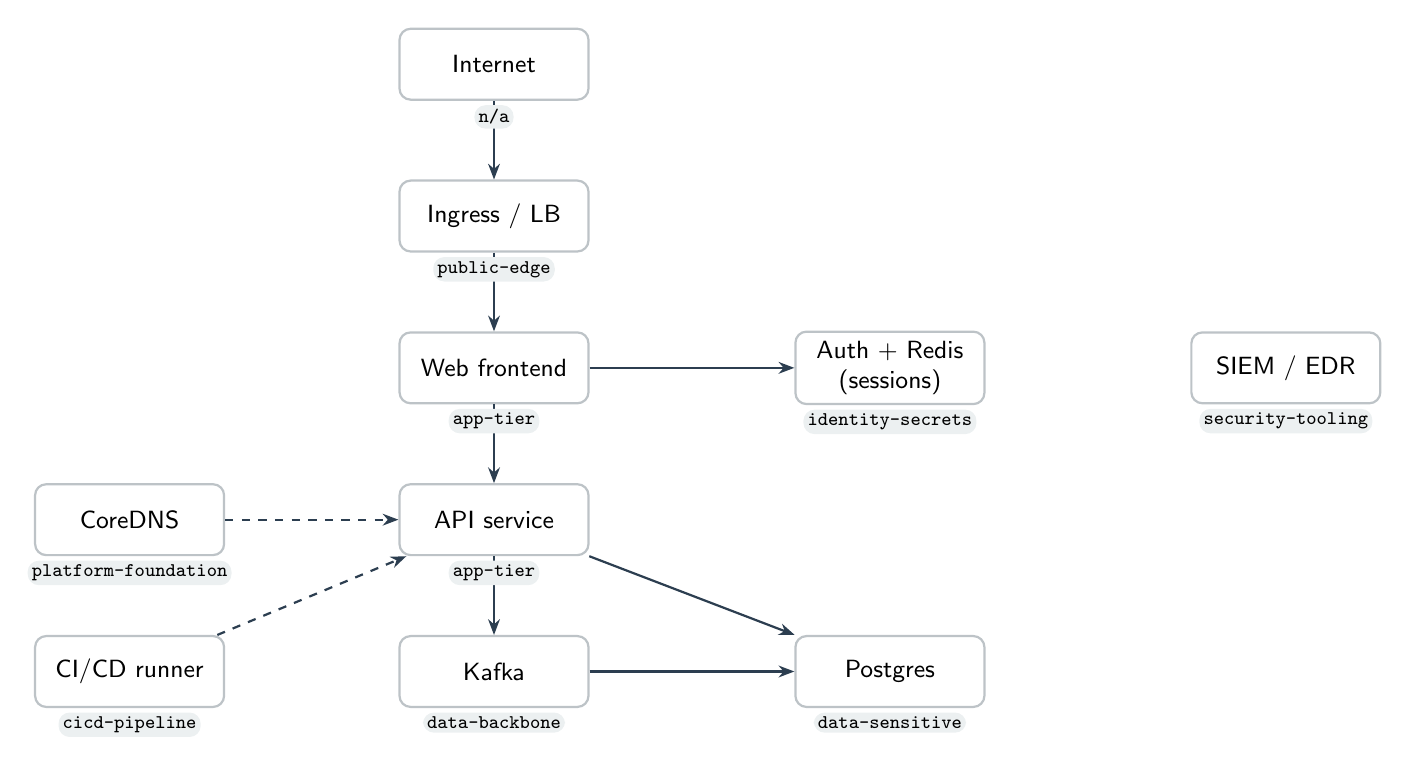
\begin{tikzpicture}[
  font=\sffamily\small,
  node distance=10mm and 14mm,
  box/.style={draw=rule,rounded corners,fill=white,minimum height=9mm,minimum width=24mm,align=center,thick},
  edge/.style={-{Stealth[length=2mm]},draw=infoblue,thick},
  tag/.style={font=\ttfamily\scriptsize,fill=tagbg,inner sep=1.5pt,rounded corners}
]
\node[box] (net) {Internet};
\node[box,below=of net] (ing) {Ingress / LB};
\node[box,below=of ing] (web) {Web frontend};
\node[box,right=26mm of web] (auth) {Auth + Redis\\(sessions)};
\node[box,below=of web] (api) {API service};
\node[box,below=of api] (kafka) {Kafka};
\node[box,right=26mm of kafka] (pg) {Postgres};
\node[box,left=22mm of api] (dns) {CoreDNS};
\node[box,left=22mm of kafka] (cicd) {CI/CD runner};
\node[box,right=26mm of auth] (siem) {SIEM / EDR};

\draw[edge] (net) -- (ing);
\draw[edge] (ing) -- (web);
\draw[edge] (web) -- (api);
\draw[edge] (web) -- (auth);
\draw[edge] (api) -- (kafka);
\draw[edge] (api) -- (pg);
\draw[edge] (kafka) -- (pg);
\draw[edge,dashed] (cicd) -- (api);
\draw[edge,dashed] (dns) -- (api);

\node[tag,below=0.5mm of net.south] {n/a};
\node[tag,below=0.5mm of ing.south] {public-edge};
\node[tag,below=0.5mm of web.south] {app-tier};
\node[tag,below=0.5mm of auth.south] {identity-secrets};
\node[tag,below=0.5mm of api.south] {app-tier};
\node[tag,below=0.5mm of kafka.south] {data-backbone};
\node[tag,below=0.5mm of pg.south] {data-sensitive};
\node[tag,below=0.5mm of dns.south] {platform-foundation};
\node[tag,below=0.5mm of cicd.south] {cicd-pipeline};
\node[tag,below=0.5mm of siem.south] {security-tooling};
\end{tikzpicture}%
}
\caption{Archetype-based reference implementation; each node carries an optional
\code{asset-archetype} tag that resolves to an asset security-impact profile.}
\label{fig:arch}
\end{figure}

\begin{table}[H]
\centering
\renewcommand{\arraystretch}{1.3}
\setlength{\tabcolsep}{4pt}
\footnotesize
\begin{tabular}{l l c c c c r}
\toprule
\textbf{CVE} & \textbf{Resource (archetype)} & \textbf{Classical} & \textbf{EPSS} & \textbf{IRV} & \textbf{PAIN} & \textbf{Remediation} \\
\midrule
CVE-2026-xxx1 & ingress \tagn{(public-edge)}        & \cellcolor{crit!25}CRITICAL & 0.97 & yes & \cellcolor{high!35}N4 & 4 days \\
CVE-2026-xxx2 & payments-db \tagn{(data-sensitive)} & \cellcolor{crit!25}CRITICAL & 0.94 & yes\,(t) & \cellcolor{high!35}N4 & 4 days \\
CVE-2026-xxx3 & redis \tagn{(identity-secrets)}     & \cellcolor{high!25}HIGH     & 0.50 & no  & \cellcolor{high!35}N4 & 8 days \\
CVE-2026-xxx4 & kafka \tagn{(data-backbone)}        & \cellcolor{low!30}LOW       & 0.76 & no  & \cellcolor{med!35}N3 & 32 days \\
CVE-2026-xxx5 & web \tagn{(app-tier)}               & \cellcolor{med!35}MEDIUM    & 0.20 & yes & \cellcolor{med!35}N3 & 128 days \\
CVE-2026-xxx6 & coredns \tagn{(platform-foundation)}& \cellcolor{med!35}MEDIUM    & 0.08 & no  & \cellcolor{low!30}N2 & 192 days \\
\bottomrule
\end{tabular}
\caption{Sample VDR scan output (fictional data, placeholder CVE IDs; Class~C, single-agency). PAIN is
computed from the effective CR/IR/AR after the intended-use ceiling is applied
and the CVE impact vector; the deadline is
$M[\text{C}][\text{PAIN}][\text{column}]$. The IRV column is evaluated \emph{per
finding} via the companion finding-level model; (t) marks transitive payload
exposure. CVE-2026-xxx2 is FedRAMP's canonical case: a content-triggered
(SQL-injection-class) finding on a datastore that is not internet-accessible is
still IRV because this sample assumes no current $P_0$ prevention assertion,
tightening the deadline to 4 days. CVE-2026-xxx4 --- a \emph{Low}
vendor severity that yields N3 (a single availability High/High alignment;
Example~4) --- stays NIRV because its
vulnerable parser sits on the inter-broker replication surface, which receives no
internet-derived data.}
\label{tab:scan}
\end{table}

\subsection{Multi-agency, Class D}
Figure~\ref{fig:archd} is a shared, multi-tenant platform serving \emph{several}
agencies at the highest assurance (Class~D). Its shared components carry more than
one agency's data, so they are tagged multi-agency (here via the cluster default,
with single-agency tenant workloads tagged as the exceptions). Table~\ref{tab:scand}
shows the result: the same families of flaws now remediate in \emph{hours}.

\begin{figure}[H]
\centering
\resizebox{\textwidth}{!}{%
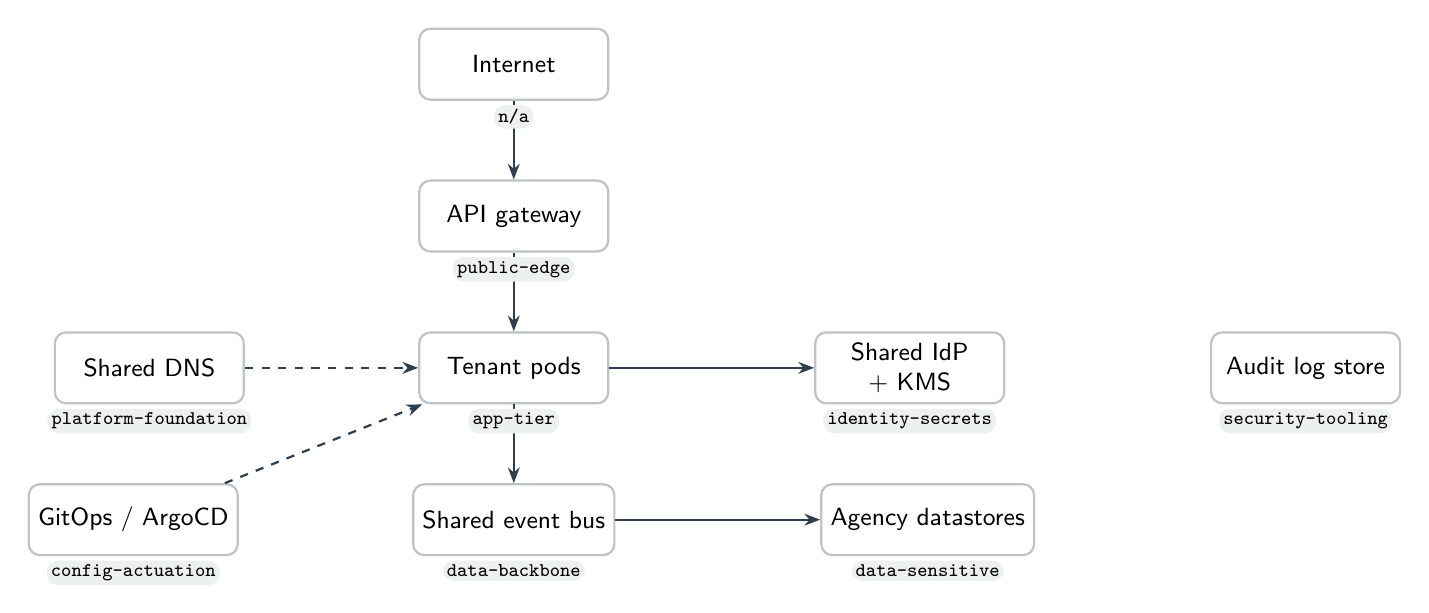
\begin{tikzpicture}[
  font=\sffamily\small,
  node distance=10mm and 14mm,
  box/.style={draw=rule,rounded corners,fill=white,minimum height=9mm,minimum width=24mm,align=center,thick},
  edge/.style={-{Stealth[length=2mm]},draw=infoblue,thick},
  tag/.style={font=\ttfamily\scriptsize,fill=tagbg,inner sep=1.5pt,rounded corners}
]
\node[box] (net) {Internet};
\node[box,below=of net] (gw) {API gateway};
\node[box,below=of gw] (app) {Tenant pods};
\node[box,right=26mm of app] (idp) {Shared IdP\\+ KMS};
\node[box,below=of app] (bus) {Shared event bus};
\node[box,right=26mm of bus] (db) {Agency datastores};
\node[box,left=22mm of app] (dns) {Shared DNS};
\node[box,left=22mm of bus] (argo) {GitOps / ArgoCD};
\node[box,right=26mm of idp] (audit) {Audit log store};

\draw[edge] (net) -- (gw);
\draw[edge] (gw) -- (app);
\draw[edge] (app) -- (idp);
\draw[edge] (app) -- (bus);
\draw[edge] (bus) -- (db);
\draw[edge,dashed] (dns) -- (app);
\draw[edge,dashed] (argo) -- (app);

\node[tag,below=0.5mm of net.south] {n/a};
\node[tag,below=0.5mm of gw.south] {public-edge};
\node[tag,below=0.5mm of app.south] {app-tier};
\node[tag,below=0.5mm of idp.south] {identity-secrets};
\node[tag,below=0.5mm of bus.south] {data-backbone};
\node[tag,below=0.5mm of db.south] {data-sensitive};
\node[tag,below=0.5mm of dns.south] {platform-foundation};
\node[tag,below=0.5mm of argo.south] {config-actuation};
\node[tag,below=0.5mm of audit.south] {security-tooling};
\end{tikzpicture}%
}
\caption{Multi-agency reference architecture; shared components serve several
agencies and are tagged multi-agency.}
\label{fig:archd}
\end{figure}

\begin{table}[H]
\centering
\renewcommand{\arraystretch}{1.3}
\setlength{\tabcolsep}{4pt}
\footnotesize
\begin{tabular}{l l c c c c r}
\toprule
\textbf{CVE} & \textbf{Resource (archetype)} & \textbf{Classical} & \textbf{EPSS} & \textbf{IRV} & \textbf{PAIN} & \textbf{Remediation} \\
\midrule
CVE-2026-yyy1 & gateway \tagn{(public-edge)}         & \cellcolor{crit!25}CRITICAL & 0.90 & yes & \cellcolor{crit!30}N5 & 12 hours \\
CVE-2026-yyy2 & shared-idp \tagn{(identity-secrets)} & \cellcolor{crit!25}CRITICAL & 0.95 & no  & \cellcolor{crit!30}N5 & 1 day \\
CVE-2026-yyy3 & event-bus \tagn{(data-backbone)}     & \cellcolor{low!30}LOW       & 0.80 & yes\,(t) & \cellcolor{high!35}N4 & 2 days \\
CVE-2026-yyy4 & agency-db \tagn{(data-sensitive)}    & \cellcolor{high!25}HIGH     & 0.40 & no  & \cellcolor{crit!30}N5 & 8 days \\
CVE-2026-yyy5 & tenant-pod \tagn{(app-tier)}         & \cellcolor{med!35}MEDIUM    & 0.10 & no  & \cellcolor{med!35}N3 & 64 days \\
CVE-2026-yyy6 & shared-dns \tagn{(platform-foundation)} & \cellcolor{med!35}MEDIUM & 0.05 & no  & \cellcolor{low!30}N2 & 192 days \\
\bottomrule
\end{tabular}
\caption{Sample VDR scan output (fictional data, placeholder CVE IDs; Class~D, multi-agency). Multi-agency
scope escalates Disruptive/Debilitating findings, and Class~D carries the tightest
deadlines --- an internet-facing exploitable flaw on the shared edge remediates in
\textbf{12 hours} (CVE-2026-yyy1). CVE-2026-yyy3 shows a \emph{Low} vendor severity
at N4 remediating in \textbf{2 days}: a content-triggered DoS in
message-payload parsing on the shared backbone is transitively internet-reachable
(t) through the tenant pods, even though the bus itself is not internet-accessible;
the sample assumes no current $P_0$ assertion covers that trigger.
A confidentiality leak on shared DNS (CVE-2026-yyy6) stays N2 and NIRV ---
``Narrow'' does not escalate with scope.}
\label{tab:scand}
\end{table}

\section{Relationship to CISA BOD 26-04}
\label{sec:bod}
The VDR/VER rule is FedRAMP's implementation of CISA Binding Operational
Directive~26-04.\footnote{CISA, \emph{Binding Operational Directive 26-04}, 2026-06-10.
The VDR rule lists it as the mandating authority, with optional adoption from
2026-07-04, obtain/maintain from 2026-12-07, and grace ending 2027-03-07.} FedRAMP
adopts the directive's \emph{philosophy} --- move remediation prioritization off raw
CVSS base scores and onto exploitability and mission impact --- but substitutes its
own instruments for the directive's pillars:

\begin{table}[H]
\centering
\renewcommand{\arraystretch}{1.25}
\footnotesize
\begin{tabular}{>{\raggedright\arraybackslash}p{0.30\textwidth} >{\raggedright\arraybackslash}p{0.30\textwidth} >{\raggedright\arraybackslash}p{0.30\textwidth}}
\toprule
\textbf{BOD 26-04 pillar} & \textbf{FedRAMP VDR/VER instrument} & \textbf{Status} \\
\midrule
SSVC drives prioritization & \textbf{PAIN} (Potential Agency Impact, N1--N5) & SSVC not named; PAIN replaces it \\
VEX communicates exploitability & \textbf{LEV} (exploitation) + disposition (\S\ref{sec:vex}) & VEX not named; role split across LEV and VER disposition \\
CSAF machine-readable advisories & VER JSON reporting (\S\ref{sec:vex}) & format unspecified; CycloneDX VEX proposed (companion) \\
KEV catalog due dates & \texttt{VDR-TFR-KEV} (defers to CISA dates) & retained intact; also consumed as a LEV input \\
(none) & \textbf{IRV/NIRV} and Certification \textbf{Class} & added as timeframe axes \\
\bottomrule
\end{tabular}
\caption{FedRAMP keeps BOD~26-04's intent but swaps SSVC$\,\rightarrow\,$PAIN and
VEX$\,\rightarrow\,$LEV${+}$disposition, retains KEV, and adds reachability and Class.}
\end{table}

The first row is the deviation that shapes this memo. Because FedRAMP chose
\emph{PAIN} rather than SSVC, an SSVC-based prioritizer does not by itself satisfy the
rule --- and FedRAMP publishes PAIN's \emph{output} buckets and the timeframe table
but not the \emph{classifier} that produces an N-level. That gap is exactly what
Section~\ref{sec:math} fills, which is why this method is expressed in CVSS
Environmental terms (the missing input was PAIN, not an exploitability score) rather
than in SSVC. The directive's other instruments retain narrower roles: this memo
consumes the \emph{KEV catalog} directly as one input to LEV
(Section~\ref{sec:remediation}) --- arguably a cleaner story than substituting for
it, since BOD~26-04's own exploitation instrument is kept intact rather than
replaced by a derived signal --- while VEX carries the post-detection
\emph{disposition} of each finding (Section~\ref{sec:vex}). Neither SSVC nor VEX is
mandated by the rule by name.

\section{Assigning the asset security-impact profile}
\label{sec:archetypes}
\begin{plain}
The PAIN formula requires an uncapped, three-dimensional CR/IR/AR profile for each
affected asset; it does not require a particular taxonomy or metadata key. A CSP
can assign the three objectives directly, derive them from a role-based archetype
catalog, or use another governed mapping. Whatever the method, it must preserve the
ability to express mixed vectors such as H/M/L and retain why each objective was
assigned.
\end{plain}
The model in Section~\ref{sec:math} is only as good as the CR/IR/AR assignment that
feeds it. A conforming implementation \rfckw{must} resolve every affected asset to
an asset security-impact profile, \rfckw{must} support independent CR, IR, and AR
assignments, and \rfckw{should} retain the derivation method, source evidence,
objective-specific rationale, policy version, and any override. This is the
normative input contract. How a CSP produces the vector is provider-governed.

\paragraph{Role-based archetype mapping.}
One strong derivation method is to sort systems into a short list of
\emph{archetypes} --- a database, a login service, a cache, a message bus, and so
on. Each archetype maps to a pre-filled security-impact profile. The mapping asks
narrow questions that architecture and inventory can help verify: does the asset
control other systems, hold credentials, authenticate users, store sensitive data,
or support several services?

A reviewer can then check both parts of the decision: whether the asset performs
the stated role and whether that role maps to the right CR/IR/AR requirements
inside the CSO. Archetypes do not remove human judgment, but they make the
architectural rationale visible, reusable, and harder to manipulate. Not every
asset will fit cleanly, so a CSP using this method \rfckw{may} define custom roles,
adjust its mappings, or make an evidenced per-asset override. The catalog in
Appendix~\ref{app:catalog} is one example derivation, not the PAIN classification
standard.

\paragraph{Direct per-objective assignment.}
A CSP \rfckw{may} instead assign CR, IR, and AR directly from a governed component
assessment. Direct assignment is fully conforming when the three objectives remain
independently selectable and the evidence and rationale are retained. It is
especially useful where a component does not fit a reusable role class or where
the provider already maintains an authoritative, objective-specific asset
classification. The method does not force CR, IR, and AR to be equal.

A simpler but less informative conforming implementation is to tag assets directly
with a scalar \code{asset-value}. Under that approach,
\code{H} or \code{High} maps to static \code{CR:H/IR:H/AR:H}; \code{M},
\code{Medium}, or \code{Moderate} maps to \code{CR:M/IR:M/AR:M}; and \code{L} or
\code{Low} maps to \code{CR:L/IR:L/AR:L}. This schema is easy to implement and
may be sufficient for smaller or more homogeneous estates. Its tradeoff is that it
states the conclusion without recording why: every security requirement moves
together, and the label does not separately explain the asset's confidentiality,
integrity, and availability needs. A scalar value \rfckw{should not} be the only
assignment interface: an implementation should permit an asset to graduate to an
independent vector without changing the scoring method.


\begin{quote}\itshape
The archetype catalog in Appendix~\ref{app:catalog} illustrates one way to derive
asset security-impact profiles. A conforming implementation does not have to use
it, use the word ``archetype,'' or expose an \code{asset-archetype} key. If a CSP
does use the catalog, it \rfckw{must} derive assignments from the roles, trust
relationships, control functions, and consequences inside its own CSO architecture.
Each CSP \rfckw{should} own and justify its mappings. The agency-specific FIPS~199
and information-type context belongs in the separately governed Security
Requirements ceiling. Two providers can legitimately derive different profiles
for the same software because it performs different roles; two agency deployments
can retain the same uncapped profile while resolving different effective
requirements.
\end{quote}

For the illustrative role-based catalog, the classification rule we recommend is
\emph{control-plane lens first}: if an
asset can deploy, orchestrate, hold cross-estate credentials, or actuate
configuration, classify it by that control function regardless of the data it
stores; otherwise classify by the data it holds. The same physical software lands
in different archetypes by role --- an in-memory store used as a cache is
\code{app-tier}, the same software used as a session/token store is
\code{identity-secrets}, and used as a job broker is \code{data-backbone}.

For Kubernetes estates, the multi-agency flag can be resolved most-specific-first:
workload label, then namespace label, then cluster default. Other deployment
models should apply the same rule to their own asset, boundary, and provider-default
metadata.

\section{Applicability and the disposition via Vulnerability Exploitability eXchange (VEX)}
\label{sec:vex}
\begin{plain}
Scoring says how bad a finding is and how fast to fix it. But a scanner's hit is not
yet a confirmed problem: the flagged code may not be present, may never run, may need
a configuration nobody set, or may already be neutralized by a control. Deciding which
is the \emph{disposition} step --- and it can only happen \emph{after} a finding is
detected, because you cannot pre-judge factors specific to a vulnerability you have not
yet seen. This section places that step in the method and names the kind of artifact
that records it: VEX.
\end{plain}

The PAIN derivation in Sections~\ref{sec:math} and~\ref{sec:remediation} is
deterministic: given the asset's CR/IR/AR, the VER axes, and the configured
thresholds, the N-level and deadline follow by formula. Disposition answers a
different question: whether the scanner finding is actually exploitable in this
running environment. That requires evidence about the specific vulnerability and
deployment --- for example, whether the affected code is present, reachable,
configured, or already neutralized by a compensating control. The analysis may be
automated, but it happens after detection because those facts are finding-specific.

\paragraph{Where FedRAMP requires it.} VER requires three things relevant here:
evaluate whether a scanner finding is real, record the per-finding disposition, and
track vulnerabilities that are accepted rather than remediated. The FedRAMP clauses
behind those duties are \code{VER-EVA-EFP}, \code{VER-EVA-AIA},
\code{VER-RPT-VDT}, and \code{VER-TFR-MAV}/\code{VER-RPT-AVI}. VER makes the
disposition step mandatory, but it does not prescribe a carrier format. The
\emph{Vulnerability Exploitability eXchange} (VEX) is a standardized,
machine-readable, signable artifact for carrying those assertions.

\paragraph{Two outcomes.} A disposition resolves a finding onto one of two tracks:
\begin{itemize}[leftmargin=1.5em,nosep,topsep=3pt]
\item \textbf{Not truly affected} --- suppressed with a machine-readable
  \emph{justification} (component or vulnerable code not present, code not reachable,
  exploitation requires a configuration that is not set, or a compensating control is
  already in place).
\item \textbf{Affected but remediation will be late} --- under VER's tight clocks a
  provider \rfckw{may} be unable to patch before the deadline; the finding is recorded
  as \emph{accepted}, with an attested mitigation and a planned response.
\end{itemize}

\paragraph{A disposition overlay, not a re-score.} Disposition does not change the
arithmetic. Every detected finding is scored as in Section~\ref{sec:math}; a VEX
assertion then moves the finding from the active remediation queue into a suppressed or
accepted set \emph{while its computed PAIN is retained}. Keeping the would-be PAIN on
record makes every suppression auditable and reversible --- the safeguard the Security
Considerations (Section~\ref{sec:seccon}) call for: a downgrade by disposition is
visible, attributable, and can be revisited if the assertion is later contradicted.

\paragraph{A distinct axis.} Applicability (VEX) is orthogonal to
exploitation-likelihood (LEV, Section~\ref{sec:remediation}). LEV asks \emph{how likely
is this vulnerability to be exploited in the wild}; VEX asks \emph{is this product, as
deployed, affected at all}. A finding can be likely-exploitable in general yet
\code{not\_affected} here because the vulnerable path is unreachable. The two are
evaluated independently and \rfckw{must not} be collapsed into one.

\paragraph{Guardrails.} Because a disposition only ever \emph{lowers} apparent risk ---
and the more so once the determination is automated --- the governing controls matter as
much as the analysis. Absent sufficient evidence a finding \rfckw{must} remain affected,
honoring \code{VER-EVA-AIA}; and the evidence required to suppress \rfckw{should} scale
with the retained PAIN, so a KEV-class, internet-reachable, high-$N$ finding demands far
stronger corroboration --- and human review --- than a low-$N$ internal one. Every
disposition \rfckw{should} cite the evidence it rests on and be signed, so it is
reproducible and attributable; and it \rfckw{should} carry a timestamp and be
re-evaluated when the image, configuration, or control it relied on changes, so a
suppression cannot outlive the condition that justified it.

\section{Determinism, governance, and defensibility}
\begin{itemize}[leftmargin=1.4em]
\item \textbf{Determinism.} Given the same (CVE vector, effective
  security-impact profile, VER axes), the method yields the same PAIN and deadline
  on every run and for every analyst.
\item \textbf{Governed asset inputs.} An asset needs an uncapped
  security-impact profile, and each finding needs an affected-agency scope. The
  profile may be assigned directly or resolved from governed metadata such as an
  archetype; the intended-use ceiling is resolved separately. Finding-specific
  cross-component evidence may identify a different consequence context without
  changing the published CVE vector.
\item \textbf{Governed calibration.} The High-centered PAIN normalization, word
  thresholds (Eq.~\eqref{eq:word}), and EPSS threshold are governed parameters and
  \rfckw{must} live in governed configuration, not in ad-hoc cluster state.
\item \textbf{Auditability.} Each finding can carry the full derivation: the
  uncapped profile, its derivation method, source and rationale, the ceiling,
  effective CR/IR/AR, $S$, the word, the scope, and the selected matrix cell.
\end{itemize}

\section{Security Considerations}
\label{sec:seccon}
The method trusts each asset's resolved security-impact profile: if someone
understates a critical component, its flaws will look smaller than they really are.
Its integrity therefore depends on the trustworthiness of the profile derivation
and the VER axes (EPSS / KEV membership / reachability). Any assignment or override
that improperly \emph{lowers} a profile is a downgrade attack; the fail-safe default
and governed calibration mitigate accidental under-classification, but profile
inputs \rfckw{should} be controlled like any other security setting. Role-based
archetypes can narrow but do not eliminate this risk: a claimed role can be compared
with architecture, data flows, identity permissions, and inventory. Direct
per-objective assignment can be equally defensible when it retains that evidence;
a scalar value label ordinarily provides less to check. Finally, the method does
not detect vulnerabilities; it prioritizes the output of a scanner and inherits
that scanner's coverage and accuracy.

\section{Conclusion}
FedRAMP VDR/VER specifies the vocabulary and the axes of vulnerability
prioritization but leaves the classifier unspecified. That classifier need not be
invented: the CVSS Environmental metric group already encodes ``re-weight impact by
what is at stake,'' which is precisely the agency-impact question. By assigning each
asset an independently dimensional security-impact profile and evaluating the two
VER axes, a provider obtains a
deterministic, auditable, and standards-grounded PAIN and remediation deadline for
every finding. A CSP may use direct per-objective assessment, a governed
classification system, or another deterministic method. We recommend role-based
archetypes as a strong starting point because they record what an asset does and
expose how its requirements were derived. A scalar asset-value label remains a
conforming fallback, but it forces CR/IR/AR to move together and records the
conclusion with less evidence behind it. We offer the example archetype catalog not
as a required taxonomy or standard but as one existence proof.

A companion proposal, \emph{A Finer Exploitability Gradation (VLEV) for FedRAMP
VDR/VER}, separately explores tightening the exploitability axis. It is kept out of
this memo deliberately: this memo's scope is meeting FedRAMP's requirements as they
stand today, not changing them. A second companion, \emph{A CycloneDX VEX Profile for
FedRAMP VDR/VER Disposition and Response}, specifies the machine-readable format
for the disposition step of Section~\ref{sec:vex}.

\appendix
\section{Example archetype-to-profile catalog}
\label{app:catalog}
Illustrative only (see Section~\ref{sec:archetypes}). This catalog demonstrates one
role-based way to derive asset security-impact profiles. A CSP may use it as a
starting point, define a different taxonomy, assign the three objectives directly,
or use another governed method.

\begin{table}[H]
\centering
\renewcommand{\arraystretch}{1.2}
\footnotesize
\setlength{\tabcolsep}{5pt}
\begin{tabular}{l l c c c >{\raggedright\arraybackslash}p{0.34\textwidth}}
\toprule
\textbf{Example archetype} & \textbf{Lens} & \textbf{CR} & \textbf{IR} & \textbf{AR} & \textbf{Typical members} \\
\midrule
\code{cicd-pipeline}      & control & H & H & H & build/deploy runners, artifact signing, registries \\
\code{orchestrator}       & control & H & H & H & control plane, etcd, scheduler, coordination \\
\code{config-actuation}   & control & H & H & H & IaC/GitOps, schema registry, admin/migration \\
\code{identity-secrets}   & control & H & H & H & IdP/SSO, KMS, secrets managers, session stores \\
\code{security-tooling}   & control & H & H & M & scanners, SIEM, EDR, runtime security \\
\code{change-record}      & control & M & M & M & ITSM/ticketing (record only) \\
\code{platform-foundation}& control & L & H & H & DNS, NTP, service discovery, L4 internal LBs (metadata only) \\
\code{data-sensitive}     & data    & H & H & H & PII/CUI datastores \\
\code{data-backbone}      & data    & H & H & H & payload queues and brokers, the system-of-record DB \\
\code{telemetry-backbone} & data    & M & M & M & metrics/trace pipelines, telemetry queues, event buses carrying no agency payload \\
\code{app-tier}           & data    & M & M & M & stateless services, APIs, UIs, caches \\
\code{batch-analytics}    & data    & M & M & L & ETL, reporting, analytics jobs \\
\code{public-edge}        & data    & M & M & H & TLS-terminating L7 edge: ingress, API gateways, public web \\
\code{passthrough-edge}   & data    & L & L & H & L4/SNI passthrough load balancers (no TLS termination) \\
\code{internal-tooling}   & data    & L & L & L & dashboards, metrics/log agents \\
\code{dev-test}           & data    & L & L & L & non-production \\
\midrule
\code{unclassified}       & ---     & H & H & H & fail-safe default for untagged assets \\
\bottomrule
\end{tabular}
\end{table}

Three assignments deserve their reasoning on the record. First, \code{data-backbone}
is reserved for components that carry agency payload data; a bus that moves only
metrics, traces, and heartbeats is \code{telemetry-backbone}, one grade lower on
every dimension. Routing payload data through a telemetry bus is a
misclassification finding, not a reason to keep every bus at High. Second, the
availability grades split deliberately between the edge and the application tier.
\code{public-edge} keeps AR High because a CVE-grade denial of service hits every
replica at once---redundancy defends against hardware failure, not against a flaw
shared by the whole class---and an edge-class outage closes the front door for
every user. \code{app-tier} sits at Medium because its blast radius is one service
degrading. An availability-only High CVE is Disruptive in both cases under the
compound-impact boundary, but High AR gives the edge the larger scalar and can
combine with a second affected dimension to cross into Debilitating. Third, the
edge itself is split by what it
does with traffic. \code{public-edge} names the TLS-terminating L7 edge --- in
practice, almost every modern ingress, gateway, or public web front --- and
carries CR and IR at Medium: a terminating edge holds private keys and session
material and sees every payload in flight, so a memory-disclosure flaw there is
key and token theft, not reconnaissance. \code{passthrough-edge} is the
deliberate opt-in for an edge that never terminates --- an L4 or SNI passthrough
that routes payload but holds none --- where CR and IR genuinely drop to Low.
The stronger values sit on the default-sounding name on purpose: an edge tagged
\code{public-edge} out of habit should overrate, not underrate. Where
termination is handled by a managed cloud load balancer whose keys never enter
the boundary, the passthrough tag is the honest one --- the terminating
component sits on the provider's side of the shared-responsibility line.

\section{Remediation deadline matrices}
\label{app:matrix}
Days; $0.5 = 12$ hours. Columns in order LEV+IRV / LEV+NIRV / NLEV. PAIN-1 has no
FedRAMP deadline (any class). The day counts below are reproduced \emph{verbatim}
from FedRAMP's published \textbf{VDR-TFR-PVR} table;\footnote{FedRAMP,
\emph{Vulnerability Detection and Response (VDR)}, provider rule, requirement
\texttt{VDR-TFR-PVR}. Generated markdown pinned at \vdrcite{} (commit of 2026-06-24);
accessed 2026-06-27. Mandated by CISA BOD~26-04; FedRAMP may revise the values.}
Classes~A and~B share one schedule. The only provider-side choice here is which
Certification Class the offering commits to --- not the numbers.

\begin{table}[H]
\centering
\footnotesize
\renewcommand{\arraystretch}{1.2}
\begin{tabular}{l ccc @{\hspace{2em}} ccc @{\hspace{2em}} ccc}
\toprule
& \multicolumn{3}{c}{\textbf{Class A / B}} & \multicolumn{3}{c}{\textbf{Class C}} & \multicolumn{3}{c}{\textbf{Class D}} \\
\cmidrule(lr){2-4}\cmidrule(lr){5-7}\cmidrule(lr){8-10}
\textbf{PAIN} & L+I & L+N & NLEV & L+I & L+N & NLEV & L+I & L+N & NLEV \\
\midrule
N5 & 4  & 8   & 32  & 2  & 4   & 16  & 0.5 & 1  & 8  \\
N4 & 8  & 32  & 64  & 4  & 8   & 64  & 2   & 8  & 32 \\
N3 & 32 & 64  & 192 & 16 & 32  & 128 & 8   & 16 & 64 \\
N2 & 96 & 160 & 192 & 48 & 128 & 192 & 24  & 96 & 192 \\
\bottomrule
\end{tabular}

\vspace{0.5em}
\begin{minipage}{0.95\textwidth}
\footnotesize
\emph{Note:} Values are days measured from \emph{completed evaluation}
(\texttt{VDR-TFR-PVR} runs its timeframes from evaluation, not detection) within
which the finding \rfckw{should} be remediated, fully mitigated, or at least
partially mitigated to a lower PAIN rating; $0.5$ represents 12 hours.
\end{minipage}
\end{table}

\section{Explicit design opinions (calibratable choices)}
\label{app:opinions}
Everything in this section is a \emph{judgment call} we made --- not something
FedRAMP or CVSS dictates. We collect them in one place so reviewers can challenge
each one, and so any adopter knows exactly which dials are theirs to turn. None of
these is load-bearing for the \emph{method}; they are the parameters the method runs
on. Each item below names the value we use, why, and the fact that an implementation
\rfckw{may} change it.

\begin{enumerate}[leftmargin=1.7em]
\item \textbf{High-centered PAIN normalization, $D_H=0.995904$.}
  PAIN retains the pre-cap aggregate $U$ and normalizes it by the maximum attainable
  all-High-impact/all-High-requirement value (Eqs.~\ref{eq:dh}--\ref{eq:s}). The
  initial publication used the CVSS MISS cap, $0.915$, as both cap and denominator.
  Because $0.915$ represents all-High impacts at \emph{Medium} requirements, that
  baseline overstated where High-requirement states sat on PAIN's full attainable
  scale and erased distinctions above the cap. The High-centered denominator closes
  that methodology gap without changing a published CVSS vector or score.
\item \textbf{PAIN word thresholds $(\theta_1,\theta_2,\theta_3) =
  (0.28115159694107,\,0.56230319388214,\,0.933)$.}
  These cut points turn $S$ into Minimal/Narrow/Disruptive/Debilitating
  (Eq.~\ref{eq:word}). The initial publication began with
  $(0.25,\,0.55,\,0.80)$. We were willing to revise those policy values, but did not
  want to choose replacements merely to fit a preferred histogram. The companion
  paper \href{https://stackarmor.github.io/rfc-fedramp-vdr/vdr-pain-calibration.pdf}
  {\emph{Calibrating PAIN Without Abandoning CVSS}} documents the data-backed
  method used instead: define consequence anchors, exhaustively enumerate all 729
  discrete impact/requirement states, and validate the result against anonymized
  operational datasets. An adopter \rfckw{should} revalidate the governed values
  against its own rated findings rather than target a desired percentage in each
  word bucket. A CSP \rfckw{may} adopt different thresholds based on its own
  documented risk evaluation, but the alternative \rfckw{should} define its word
  semantics first, enumerate the supported state space, validate boundary
  consequences, disclose the active policy to affected agencies, and version the
  complete calibration. Thresholds \rfckw{must not} be changed ad hoc after seeing
  a finding's deadline. They should also remain independent of Certification Class:
  Class selects the response commitment after potential impact is derived.
\item \textbf{Compound impact is a proxy; CWE is not a PAIN input.}
  The reference $\theta_3$ preserves at least one High-impact/High-requirement
  alignment and requires another High impact on a Moderate-or-High requirement.
  This is our auditable approximation that vulnerabilities capable of
  multidimensional loss belong in a broader consequence class before receiving the
  word Debilitating. It is not a CWE classifier. CWE is designed for weakness
  root-cause mapping, contains multiple abstraction levels, and can be missing,
  multiply mapped, or imprecise for a particular vulnerability. A provider-authored
  CWE-to-severity table would therefore add a large, contestable input with no
  stable precedence over observed CVSS impact. CWE \rfckw{may} still support
  remediation ownership, secure-development analysis, detection planning, and
  finding grouping outside the PAIN calculation.
\item \textbf{EPSS Likely-Exploitable threshold $\theta_{\text{epss}} = 0.50$.}
  The EPSS probability at or above which a finding is treated as LEV
  (Section~\ref{sec:remediation}). This memo recommends $0.50$ so vulnerabilities
  with at least an even predicted chance of exploitation enter the fast track;
  higher values produce fewer fast-track findings. FedRAMP leaves the framework
  to the provider.
\item \textbf{LEV is a union, not a blend.} A finding is Likely Exploitable if
  EPSS $\ge \theta_{\text{epss}}$, \emph{or} it is listed in the CISA KEV catalog ---
  whichever fires, with no weighting among them.
\item \textbf{Impact-only severity.} We use the CVSS-derived impact aggregate rather
  than computing the full Environmental Score; exploitability and reachability
  select the remediation column instead of influencing the PAIN row.
  Section~\ref{sec:cvss-divergence} enumerates this choice and every downstream CVSS
  component the method omits.
\item \textbf{Likelihood-only partial mitigation may use a labeled PAIN proxy.}
  FedRAMP defines partial mitigation as reducing likelihood or PAIN, while its
  timeframe and reporting workflow expresses progress through lower N-ratings.
  Section~\ref{sec:pain-proxy} retains consequence PAIN and permits a separately
  labeled residual-response proxy for verified local likelihood reduction. The
  same mitigation may also update the separately required IRV/LEV column; both
  outputs carry common provenance and are disclosed as correlated expressions of
  one control, not independent reductions. This reconciliation is ours, not a
  FedRAMP formula, and the proxy needs governed, disclosed calibration before
  operational use.
\item \textbf{CISA Vulnrichment is deliberately excluded.} Two CISA Vulnrichment
  SSVC values are natural candidate inputs: the exploitation state (as a
  LEV input) and the technical impact (as an impact floor). We adopt neither. The
  exploitation role is served by KEV membership --- the instrument BOD~26-04
  itself names --- and a technical-impact floor is rejected because an opaque,
  externally-fixed impact floor cannot coexist with the evidence-based
  Modified~C/I/A mitigation lever of Section~\ref{sec:ladder}: when a fixed floor
  and cited local evidence disagree, there is no principled precedence between
  them, and the Environmental layer already re-weights impact per deployment. EPSS
  and the KEV catalog remain the two governed threat inputs. An adopter \rfckw{may}
  reintroduce enrichment sources, at its own risk of exactly that conflict.
\item \textbf{Modifications lower High to Low, never to None; evidence scales with
  the PAIN reduced.} The mitigation lever of Section~\ref{sec:ladder} lets cited,
  signed evidence lower a Modified impact dimension, but never to None: a claim of
  \emph{zero} impact is an applicability claim and must travel as a VEX disposition
  (Section~\ref{sec:vex}), where it is separately governed, auditable, and
  reversible. And the evidence bar scales with the stakes --- lowering an N5 to an
  N4 demands stronger corroboration than lowering an N2 to an N1, mirroring the
  disposition guardrails. Both rules are ours, not FedRAMP's; an adopter tightening
  or relaxing them \rfckw{should} do so in governed configuration.
\item \textbf{Automatic high-availability credit is scoped by reachability.}
  Verified redundancy (replicas, required zone anti-affinity with observed spread,
  PodDisruptionBudget, automatic restart) applies \code{MA}
  High$\rightarrow$Low automatically for findings that are \emph{not}
  internet-reachable; internet-reachable findings take the step only with a
  per-finding citation explaining why the trigger cannot be repeated at line
  rate. Rationale: IRV means the attacker can re-deliver the exploit, and
  replication defends against uncorrelated failure, not a flaw every replica
  shares. An adopter \rfckw{may} tighten this (citation everywhere) or, at its
  own risk, relax the reachability carve-out; either choice belongs in governed
  configuration with the residual documented.
\item \textbf{Scope is finding-specific; hierarchical metadata is the baseline.}
  Asset, containing-boundary, and provider-default tags resolve most-specific-first
  as the operational starting point. Evidence that a finding is tenant-contained
  can keep a shared asset single-agency; evidence that its effect traverses a
  shared control plane or dependency can establish multi-agency scope. There is no
  automatic per-archetype escalation and no generic scope multiplier. The
  affected-agency basis remains explicit and operator-controlled.\par\smallskip
\item \textbf{The profile is required; an archetype is optional.} The formula
  ultimately requires a per-asset effective Security Requirements vector
  (\code{CR/IR/AR}); the upstream asset security-impact profile may come from direct
  per-objective assessment, an archetype catalog, or any governed classification
  scheme that maps deterministically to independently representable CR/IR/AR.
  No implementation is required to expose \code{asset-archetype} or any particular
  metadata key. We recommend role-based archetypes as one strong derivation method
  because they provide granularity and a clear, auditable evidence chain. The same
  software can therefore land in different example archetypes by how it is used
  (an in-memory store is \code{app-tier} as a cache,
  \code{identity-secrets} as a session store, or \code{data-backbone} as a broker).
  A scalar asset-value label is permitted as shorthand but should not be the only
  interface because it collapses all objectives to one repeated value. If an
  adopter retains an archetype taxonomy, the role-not-software-kind semantics
  should be preserved.
\item \textbf{The intended-use ceiling is separate from the asset profile.}
  Equation~\eqref{eq:effective-requirement} caps the asset's system-relative profile by
  the confirmed, dimensional federal consequence of the affected agency scope.
  This lets one CSO reuse its profile derivation policy across agency deployments without
  pretending that agency information types are intrinsic properties of a
  component. The preferred derivation retains confirmed NIST SP~800-60 information
  types; the simpler \code{min(SSO, ASO)} vector form is a documented
  approximation. An omitted ceiling preserves uncapped, conservative compatibility
  behavior but is not an evidenced agency-specific derivation.
\item \textbf{Fail-safe defaults to conservative High.} An unclassified asset defaults
  to CR/IR/AR all High so it scores loudly, rather than to a low default. ``Unknown''
  is treated as serious until classified.
\item \textbf{CVSS v3.1, not v4.0.} We build on v3.1's closed-form environmental
  formula because it provides a Modified Impact Sub-Score whose pre-cap expression
  is Eq.~\ref{eq:u}, with
  explicit CR/IR/AR multipliers. CVSS v4.0 retains CR/IR/AR but feeds them into a
  lookup-based MacroVector rather than the v3.1 formula, and it splits impact into
  Vulnerable-System (\code{VC/VI/VA}) and Subsequent-System (\code{SC/SI/SA})
  metrics. A v4.0-only finding can use the limited compatibility mapping from
  \code{VC/VI/VA} onto $C/I/A$, but Subsequent-System metrics remain reviewable
  evidence and must not disappear from the derivation record. This memo does not
  define automatic multi-target aggregation. While NVD remains v3.1-dominant, an
  implementation \rfckw{should} prefer the v3.1 vector when both are available.
\item \textbf{The example archetype-to-profile catalog and its CR/IR/AR values
  (Appendix~\ref{app:catalog}).} Illustrative only --- each CSP \rfckw{should} derive
  its security-impact profiles from component roles, trust, privilege,
  dependencies, data handling, and consequences inside its CSO architecture, then
  apply the separately governed intended-use ceiling. A 3PAO \rfckw{may} take on the
  role of validating the derivation policy and assignments during an assessment;
  however, the CSP remains ultimately responsible if an asset profile is
  understated, a vulnerability is not
  remediated in time, and it is subsequently exploited (just as in the 
  commercial world).
\item \textbf{The remediation deadline values (Appendix~\ref{app:matrix}) are
  \emph{not} ours to calibrate.} They are reproduced verbatim from FedRAMP's published
  \texttt{VDR-TFR-PVR} table (mandated by CISA BOD~26-04; see Section~\ref{sec:bod}).
  The only provider-side choice is which Certification Class (A--D) the offering
  commits to, selecting the column block; the day counts themselves are fixed by
  FedRAMP. Listed here only to mark the boundary between what we chose and what the
  rule dictates.
\end{enumerate}

\section*{Acknowledgements}
\addcontentsline{toc}{section}{Acknowledgements}
While this paper has a single official author, the underlying work, refinement,
and practical validation were a collaborative effort. It would not have been
possible without the generous help, critical feedback, and dedicated support of
various other team members at stackArmor who helped make it possible.

\section*{Normative sources}
\addcontentsline{toc}{section}{Normative sources}
\begin{itemize}[leftmargin=3.4em]
\item[{[VDR]}] FedRAMP, \emph{Vulnerability Detection and Response (VDR)}.
  Requirements cited: \texttt{VDR-TFR-PVR}, \texttt{VDR-TFR-KEV},
  \texttt{VDR-TFR-PDD/PCD/PSD}. Pinned permalink: \vdrcite{} (commit of 2026-06-24;
  generated from upstream \texttt{fedramp/rules}). Accessed 2026-06-27.
\item[{[VER]}] FedRAMP, \emph{Vulnerability Evaluation and Reporting (VER)}.
  Requirements cited: \texttt{VER-EVA-EIR}, \texttt{VER-EVA-EFP},
  \texttt{VER-EVA-AIA}, \texttt{VER-RPT-VDT}, \texttt{VER-TFR-MAV},
  \texttt{VER-RPT-AVI}. Pinned permalink: \vercite{} (commit of 2026-06-24).
  Accessed 2026-07-01.
\item[{[DEF]}] FedRAMP, \emph{FedRAMP Definitions}. Definitions cited:
  \texttt{FRD-IRV}, \texttt{FRD-LEV}, \texttt{FRD-PAI},
  \texttt{FRD-PMV}, \texttt{FRD-FMV}, and \texttt{FRD-RMV}. Pinned permalink:
  \defcite{} (commit of 2026-06-24). Accessed 2026-07-01.
\item[{[EGR]}] M.~Venne, \emph{Internet Reachability at Scale under the FedRAMP
  VDR/VER Rules}, stackArmor,
  July 2026. Companion paper specifying the reachability determination used here.
\item[{[CEILING]}] M.~Venne, \emph{Before the PAIN Equation: Deriving
  Security-Requirements Ceilings from Intended Federal Information Types},
  stackArmor, July 2026. Upstream derivation of effective CR/IR/AR.
\item[{[FIPS199]}] National Institute of Standards and Technology,
  \emph{Standards for Security Categorization of Federal Information and
  Information Systems}, FIPS PUB 199, February 2004.
\item[{[SP800-60]}] National Institute of Standards and Technology,
  \emph{Guide for Mapping Types of Information and Information Systems to Security
  Categories}, SP 800-60 Volumes I and II, Revision 1, August 2008.
\item[{[BOD]}] CISA, \emph{Binding Operational Directive 26-04}, 2026-06-10.
\item[{[KEV]}] CISA, \emph{Known Exploited Vulnerabilities (KEV) Catalog}. LEV
  input; \texttt{VDR-TFR-KEV} schedule.
\item[{[CVSS]}] FIRST, \emph{CVSS v3.1 Specification} --- Environmental metric group
  and Modified Impact Sub-Score.
\item[{[CVSS40]}] FIRST, \emph{Common Vulnerability Scoring System v4.0:
  Specification Document}. Vulnerable- and Subsequent-System impact metrics.
  \url{https://www.first.org/cvss/v4.0/specification-document}.
\item[{[CVSS40-UG]}] FIRST, \emph{CVSS v4.0 User Guide}. Vulnerable-System and
  Subsequent-System boundary guidance, including the SQL-injection example.
  \url{https://www.first.org/cvss/user-guide.html}.
\item[{[EPSS]}] FIRST, \emph{Exploit Prediction Scoring System}.
\item[{[CLASS]}] FedRAMP, \emph{Choosing a Certification Class}, Consolidated
  Rules for 2026.
  \url{https://www.fedramp.gov/2026/providers/start/class/#alignment-with-agency-use-cases}.
\item[{[IEC]}] FedRAMP, \emph{Incident Evaluation and Communication},
  Consolidated Rules for 2026.
  \url{https://www.fedramp.gov/2026/providers/20x/rules/incident-evaluation-and-communication/}.
\item[{[CWE-RCM]}] MITRE, \emph{CVE to CWE Root Cause Mapping Guidance}.
  \url{https://cwe.mitre.org/documents/cwe_usage/guidance.html}.
\end{itemize}

\end{document}
